
%% bare_conf.tex
%% V1.3
%% 2007/01/11
%% by Michael Shell
%% See:
%% http://www.michaelshell.org/
%% for current contact information.
%%
%% This is a skeleton file demonstrating the use of IEEEtran.cls
%% (requires IEEEtran.cls version 1.7 or later) with an IEEE conference paper.
%%
%% Support sites:
%% http://www.michaelshell.org/tex/ieeetran/
%% http://www.ctan.org/tex-archive/macros/latex/contrib/IEEEtran/
%% and
%% http://www.ieee.org/

%%*************************************************************************
%% Legal Notice:
%% This code is offered as-is without any warranty either expressed or
%% implied; without even the implied warranty of MERCHANTABILITY or
%% FITNESS FOR A PARTICULAR PURPOSE! 
%% User assumes all risk.
%% In no event shall IEEE or any contributor to this code be liable for
%% any damages or losses, including, but not limited to, incidental,
%% consequential, or any other damages, resulting from the use or misuse
%% of any information contained here.
%%
%% All comments are the opinions of their respective authors and are not
%% necessarily endorsed by the IEEE.
%%
%% This work is distributed under the LaTeX Project Public License (LPPL)
%% ( http://www.latex-project.org/ ) version 1.3, and may be freely used,
%% distributed and modified. A copy of the LPPL, version 1.3, is included
%% in the base LaTeX documentation of all distributions of LaTeX released
%% 2003/12/01 or later.
%% Retain all contribution notices and credits.
%% ** Modified files should be clearly indicated as such, including  **
%% ** renaming them and changing author support contact information. **
%%
%% File list of work: IEEEtran.cls, IEEEtran_HOWTO.pdf, bare_adv.tex,
%%                    bare_conf.tex, bare_jrnl.tex, bare_jrnl_compsoc.tex
%%*************************************************************************

% *** Authors should verify (and, if needed, correct) their LaTeX system  ***
% *** with the testflow diagnostic prior to trusting their LaTeX platform ***
% *** with production work. IEEE's font choices can trigger bugs that do  ***
% *** not appear when using other class files.                            ***
% The testflow support page is at:
% http://www.michaelshell.org/tex/testflow/



% Note that the a4paper option is mainly intended so that authors in
% countries using A4 can easily print to A4 and see how their papers will
% look in print - the typesetting of the document will not typically be
% affected with changes in paper size (but the bottom and side margins will).
% Use the testflow package mentioned above to verify correct handling of
% both paper sizes by the user's LaTeX system.
%
% Also note that the "draftcls" or "draftclsnofoot", not "draft", option
% should be used if it is desired that the figures are to be displayed in
% draft mode.
%
\documentclass[conference]{IEEEtran}
% Add the compsoc option for Computer Society conferences.
%
% If IEEEtran.cls has not been installed into the LaTeX system files,
% manually specify the path to it like:
% \documentclass[conference]{../sty/IEEEtran}


\usepackage[latin1]{inputenc}
\usepackage{times}
\usepackage{helvet}
%package pour les algo
\usepackage{algorithm}
\usepackage{algorithmic}
\usepackage{comment}
%\usepackage{algpseudocode}
%\pagestyle{empty}
%\newcommand{\smallitem}{\vspace*{-2mm}\item}
%\renewcommand{\baselinestretch}{0.95}
%\marginparwidth 0pt 
%\evensidemargin 2.2cm 
%\oddsidemargin 1.8cm 
%\topmargin 0cm 
%\textwidth 12cm 
%\textheight 19cm


%\makeatletter
%\renewcommand{\fnum@figure}{\textbf{\fontsize{10}{10}\selectfont\sffamily\figurename~\thefigure}}
%\renewcommand{\fnum@table}{\textbf{\fontsize{10}{10}\selectfont\sffamily\tablename~\thetable}}
%\makeatother

\begin{comment}
\newcommand{\auteur}[1]{
	\begin{center}
	{#1}
	\end{center}
}

\newcommand{\titre}[1]{
	\begin{center}
	{\large\bfseries \sffamily {#1}}
	\end{center}
}

\newcommand{\affiliation}[1]{
	\noindent
	{\small{#1}}
}
\end{comment}

\usepackage{hyperref}
\usepackage{amsmath}  % Maths
\usepackage{amsfonts} % Maths
\usepackage{amssymb}  % Maths
\usepackage{stmaryrd} % Maths (crochets doubles)

\usepackage{url}     % Mise en forme + liens pour URLs
\usepackage{array}   % Tableaux évolués

\usepackage{prettyref}
\newrefformat{def}{Def.~\ref{#1}}
\newrefformat{fig}{Fig.~\ref{#1}}
\newrefformat{pro}{Property~\ref{#1}}
\newrefformat{pps}{Proposition~\ref{#1}}
\newrefformat{lem}{Lemma~\ref{#1}}
\newrefformat{thm}{Theorem~\ref{#1}}
\newrefformat{sec}{Sect.~\ref{#1}}
\newrefformat{ssec}{Subsect.~\ref{#1}}
\newrefformat{suppl}{Appendix~\ref{#1}}
\newrefformat{eq}{Eq.~\eqref{#1}}
\def\pref{\prettyref}

\usepackage{ntheorem}
\theoremheaderfont{\fontsize{10}{10}\sffamily\bfseries}
%\newtheorem*{example}{Example}{\itshape}{}
\newtheorem{example}{Example}{\itshape}{}
\newtheorem{definition}{Definition}{\itshape}{}


\usepackage{tikz}
\newdimen\pgfex
\newdimen\pgfem
\usetikzlibrary{arrows,shapes}
%\usetikzlibrary{shadows,scopes}
%\usetikzlibrary{positioning}
%\usetikzlibrary{matrix}
%\usetikzlibrary{decorations.text}
%\usetikzlibrary{decorations.pathmorphing}



%\input{macros/macros}

% Macros générales
\def\Pint{\textsc{PINT}}

% Notations générales pour PH
\newcommand{\PH}{\mathcal{PH}}
\newcommand{\PHs}{\Sigma}
\newcommand{\PHl}{L}
\newcommand{\PHp}{\textcolor{red}{\mathcal{P}}}
\newcommand{\PHproc}{\mathcal{P}}
\newcommand{\PHa}{\PHh}
\newcommand{\PHh}{\mathcal{H}}
\newcommand{\PHn}{\mathcal{N}}

\newcommand{\PHhitter}{\mathsf{hitter}}
\newcommand{\PHtarget}{\mathsf{target}}
\newcommand{\PHbounce}{\mathsf{bounce}}
\newcommand{\PHsort}{\Sigma}

\def\f#1{\mathsf{#1}}
\def\focals{\f{focals}}
\def\play{\cdot}
\def\configs#1{\mathbb C_{#1\rightarrow a}}

\newcommand{\PHfrappeA}{\rightarrow}
\newcommand{\PHfrappeB}{\Rsh}
\newcommand{\PHfrappe}[3]{#1\PHfrappeA#2\PHfrappeB#3}
\newcommand{\PHfrappebond}[2]{#1\PHfrappeB#2}
\newcommand{\PHobjectif}[2]{\mbox{$#1\PHfrappeB^*\!#2$}}
\newcommand{\PHconcat}{::}
\newcommand{\PHneutralise}{\rtimes}

\def\PHget#1#2{{#1[#2]}}
\newcommand{\PHchange}[2]{(#1 \Lleftarrow #2)}
\newcommand{\PHarcn}[2]{\mbox{$#1\PHneutralise#2$}}
\newcommand{\PHjoue}{\cdot}

\newcommand{\PHetat}[1]{\mbox{$\langle #1 \rangle$}}

% Notations spécifiques à ce papier
\newcommand{\PHdirectpredec}[1]{\PHs^{-1}(#1)}
\newcommand{\PHpredec}[1]{\f{pred}(#1)}
\newcommand{\PHpredecgene}[1]{\f{reg}({#1})}
\newcommand{\PHpredeccs}[1]{\PHpredec{#1} \setminus \Gamma}

\newcommand{\PHincl}[2]{#1 :: #2}

\def\ctx{\varsigma}
\def\ctxOverride{\Cap}
\def\PHstate#1{\langle #1 \rangle}

\def\DEF{\stackrel{\Delta}=}
\def\EQDEF{\stackrel{\Delta}\Leftrightarrow}

\def\intervalless{<_{[]}}

%\input{macros/macros-ph}

% Notations pour le modèle de Thomas (depuis thèse)
\newcommand{\GRN}{\mathcal{GRN}}
\newcommand{\IG}{\mathcal{G}}
\newcommand{\GRNreg}[1]{\Gamma^{-1}(#1)}
\newcommand{\GRNres}[2]{\mathsf{Res}_{#1}(#2)}
\newcommand{\GRNallres}[1]{\mathsf{Res}_{#1}}
\newcommand{\GRNget}[2]{\PHget{#1}{#2}}
\newcommand{\GRNetat}[1]{\PHetat{#1}}

\def\levels{\mathsf{levels}}
\def\levelsA#1#2{\levels_+(#1\rightarrow #2)}
\def\levelsI#1#2{\levels_-(#1\rightarrow #2)}

\newcommand{\Kinconnu}{\emptyset}
\newcommand{\RRGva}[3]{#1 \stackrel{#2}{\longrightarrow} #3}
\newcommand{\RRGgi}{\mathcal{G}}
\newcommand{\RRGreg}[1]{\RRGgi_{#1}}

\tikzstyle{grn}=[every node/.style={circle,draw=black,outer sep=2pt,minimum
                size=15pt,text=black}, node distance=1.5cm]
\tikzstyle{act}=[->,draw=black,thick,color=black]
\tikzstyle{inh}=[>=|,-|,draw=black,thick, text=black,label]
\tikzstyle{inf}=[->,draw=colorinf,thick,color=colorinf]
\tikzstyle{elabel}=[fill=none,text=black, above=-2pt,%sloped,
minimum size=10pt, outer sep=0, font=\scriptsize, draw=none]
\tikzstyle{sg}=[every node/.style={outer sep=2pt,minimum
                size=15pt,text=black}, node distance=2cm]
                

%Notations pour les patterns dans cytoscape
%%%%%%%%%%%%%%%%%%%%%%%%%%%%%%%%%%%%%%%%%%%%%%%%%%%%%%%%%%%%%%%%%%%%%%%%%%%%%%%%%%%%%%%%%%%
%%%%%%%%%%%%%%%%%%%%%%%%%%%%%%%%%%%%%%%%%%%%%%%%%%%%%%%%%%%%%%%%%%%%%%%%%%%%%%%%%%%%%%%%%%%
%%%%%%%%%%%%%%%%%%Definition des éléments pour un reseau de signalisation%%%%%%%%%%%%%%%%%
\definecolor{pinegreen}{cmyk}{0.92,0,0.59,0.25}
\definecolor{royalblue}{cmyk}{1,0.50,0,0}
\definecolor{lavander}{cmyk}{0,0.48,0,0}
\definecolor{violet}{cmyk}{0.79,0.88,0,0}
\tikzstyle{sn}=[circle, draw, thin,fill=cyan!20, scale=0.8] %seed node
\tikzstyle{ps}=[rectangle, draw, thin,fill=green!20, scale=0.8] %protein de signalisation
\tikzstyle{cplx}=[square, draw, thin, fill=white!20, scale=0.7] %définition d'un complex
\tikzstyle{transl}=[diamond, draw, thin, fill=white!20, scale=0.3]
\tikzstyle{mod}=[triangle, draw, thin, fill=white!20, scale=0.3]
\tikzstyle{qgre}=[rectangle, draw, thin,fill=green!20, size=15pts]
\tikzstyle{tgrn}=[triangle, draw, thin, fill=green!20, scale=0.8]

%Ajout des arc qui ne sont pas définis dans le grn
\tikzstyle{st}=[->, draw, thin, dashed] %définition d'un state transition
\tikzstyle{inhN}=[>=|,-|,draw=colorinh,thick, text=black,label,scale=0.1]
\tikzstyle{actN}=[->,>=triangle 60,draw=coloract,thick,color=coloract,scale=0.1]





%\input{macros/macros-grn}

\usepackage{ifthen}
%\usepackage{tikz}
%\usetikzlibrary{arrows,shapes}

\definecolor{lightgray}{rgb}{0.8,0.8,0.8}
\definecolor{lightgrey}{rgb}{0.8,0.8,0.8}

\tikzstyle{boxed ph}=[]
\tikzstyle{sort}=[fill=lightgray,rounded corners]
\tikzstyle{process}=[circle,draw,minimum size=15pt,fill=white,
font=\footnotesize,inner sep=1pt]
\tikzstyle{black process}=[process, fill=black,text=white, font=\bfseries]
\tikzstyle{gray process}=[process, draw=black, fill=lightgray]
\tikzstyle{current process}=[process, draw=black, fill=lightgray]
\tikzstyle{process box}=[white,draw=black,rounded corners]
\tikzstyle{tick label}=[font=\footnotesize]
\tikzstyle{tick}=[black,-]%,densely dotted]
\tikzstyle{hit}=[->,>=angle 45]
\tikzstyle{selfhit}=[min distance=30pt,curve to]
\tikzstyle{bounce}=[densely dotted,->,>=latex]
\tikzstyle{hl}=[font=\bfseries,very thick]
\tikzstyle{hl2}=[hl]
\tikzstyle{nohl}=[font=\normalfont,thin]

\newcommand{\currentScope}{}
\newcommand{\currentSort}{}
\newcommand{\currentSortLabel}{}
\newcommand{\currentAlign}{}
\newcommand{\currentSize}{}

\newcounter{la}
\newcommand{\TSetSortLabel}[2]{
  \expandafter\repcommand\expandafter{\csname TUserSort@#1\endcsname}{#2}
}
\newcommand{\TSort}[4]{
  \renewcommand{\currentScope}{#1}
  \renewcommand{\currentSort}{#2}
  \renewcommand{\currentSize}{#3}
  \renewcommand{\currentAlign}{#4}
  \ifcsname TUserSort@\currentSort\endcsname
    \renewcommand{\currentSortLabel}{\csname TUserSort@\currentSort\endcsname}
  \else
    \renewcommand{\currentSortLabel}{\currentSort}
  \fi
  \begin{scope}[shift={\currentScope}]
  \ifthenelse{\equal{\currentAlign}{l}}{
    \filldraw[process box] (-0.5,-0.5) rectangle (0.5,\currentSize-0.5);
    \node[sort] at (-0.2,\currentSize-0.4) {\currentSortLabel};
   }{\ifthenelse{\equal{\currentAlign}{r}}{
     \filldraw[process box] (-0.5,-0.5) rectangle (0.5,\currentSize-0.5);
     \node[sort] at (0.2,\currentSize-0.4) {\currentSortLabel};
   }{
    \filldraw[process box] (-0.5,-0.5) rectangle (\currentSize-0.5,0.5);
    \ifthenelse{\equal{\currentAlign}{t}}{
      \node[sort,anchor=east] at (-0.3,0.2) {\currentSortLabel};
    }{
      \node[sort] at (-0.6,-0.2) {\currentSortLabel};
    }
   }}
  \setcounter{la}{\currentSize}
  \addtocounter{la}{-1}
  \foreach \i in {0,...,\value{la}} {
    \TProc{\i}
  }
  \end{scope}
}

\newcommand{\TTickProc}[2]{ % pos, label
  \ifthenelse{\equal{\currentAlign}{l}}{
    \draw[tick] (-0.6,#1) -- (-0.4,#1);
    \node[tick label, anchor=east] at (-0.55,#1) {#2};
   }{\ifthenelse{\equal{\currentAlign}{r}}{
    \draw[tick] (0.6,#1) -- (0.4,#1);
    \node[tick label, anchor=west] at (0.55,#1) {#2};
   }{
    \ifthenelse{\equal{\currentAlign}{t}}{
      \draw[tick] (#1,0.6) -- (#1,0.4);
      \node[tick label, anchor=south] at (#1,0.55) {#2};
    }{
      \draw[tick] (#1,-0.6) -- (#1,-0.4);
      \node[tick label, anchor=north] at (#1,-0.55) {#2};
    }
   }}
}
\newcommand{\TSetTick}[3]{
  \expandafter\repcommand\expandafter{\csname TUserTick@#1_#2\endcsname}{#3}
}

\newcommand{\myProc}[3]{
  \ifcsname TUserTick@\currentSort_#1\endcsname
    \TTickProc{#1}{\csname TUserTick@\currentSort_#1\endcsname}
  \else
    \TTickProc{#1}{#1}
  \fi
  \ifthenelse{\equal{\currentAlign}{l}\or\equal{\currentAlign}{r}}{
    \node[#2] (\currentSort_#1) at (0,#1) {#3};
  }{
    \node[#2] (\currentSort_#1) at (#1,0) {#3};
  }
}
\newcommand{\TSetProcStyle}[2]{
  \expandafter\repcommand\expandafter{\csname TUserProcStyle@#1\endcsname}{#2}
}
\newcommand{\TProc}[1]{
  \ifcsname TUserProcStyle@\currentSort_#1\endcsname
    \myProc{#1}{\csname TUserProcStyle@\currentSort_#1\endcsname}{}
  \else
    \myProc{#1}{process}{}
  \fi
}

\newcommand{\repcommand}[2]{
  \providecommand{#1}{#2}
  \renewcommand{#1}{#2}
}
\newcommand{\THit}[5]{
  \path[hit] (#1) edge[#2] (#3#4);
  \expandafter\repcommand\expandafter{\csname TBounce@#3@#5\endcsname}{#4}
}
\newcommand{\TBounce}[4]{
  (#1\csname TBounce@#1@#3\endcsname) edge[#2] (#3#4)
}

\newcommand{\TState}[1]{
  \foreach \proc in {#1} {
    \node[current process] (\proc) at (\proc.center) {};
  }
}

%%%%%%%%%%%%%%%%%%%%%%%%%%%%%%%%%%%%%%%%%%%%%%%%%%%%%%%%%%%%%%%%%
%% The following definitions are to extend the LaTeX algorithmic 
%% package with SWITCH statements and one-line structures.
%% The extension is by 
%%   Prof. Farn Wang 
%%   Dept. of Electrical Engineering, 
%%   National Taiwan University. 
%% 
\newcommand{\SWITCH}[1]{\STATE \textbf{switch} (#1)}
\newcommand{\ENDSWITCH}{\STATE \textbf{end switch}}
\newcommand{\CASE}[1]{\STATE \textbf{case} #1\textbf{:} \begin{ALC@g}}
\newcommand{\ENDCASE}{\end{ALC@g}}
\newcommand{\CASELINE}[1]{\STATE \textbf{case} #1\textbf{:} }
\newcommand{\DEFAULT}{\STATE \textbf{default:} \begin{ALC@g}}
\newcommand{\ENDDEFAULT}{\end{ALC@g}}
\newcommand{\DEFAULTLINE}[1]{\STATE \textbf{default:} }
%% 
%% End of the LaTeX algorithmic package extension.
%%%%%%%%%%%%%%%%%%%%%%%%%%%%%%%%%%%%%%%%%%%%%%%%%%%%%%%%%%%%%%%%%


% Some very useful LaTeX packages include:
% (uncomment the ones you want to load)


% *** MISC UTILITY PACKAGES ***
%
%\usepackage{ifpdf}
% Heiko Oberdiek's ifpdf.sty is very useful if you need conditional
% compilation based on whether the output is pdf or dvi.
% usage:
% \ifpdf
%   % pdf code
% \else
%   % dvi code
% \fi
% The latest version of ifpdf.sty can be obtained from:
% http://www.ctan.org/tex-archive/macros/latex/contrib/oberdiek/
% Also, note that IEEEtran.cls V1.7 and later provides a builtin
% \ifCLASSINFOpdf conditional that works the same way.
% When switching from latex to pdflatex and vice-versa, the compiler may
% have to be run twice to clear warning/error messages.






% *** CITATION PACKAGES ***
%
%\usepackage{cite}
% cite.sty was written by Donald Arseneau
% V1.6 and later of IEEEtran pre-defines the format of the cite.sty package
% \cite{} output to follow that of IEEE. Loading the cite package will
% result in citation numbers being automatically sorted and properly
% "compressed/ranged". e.g., [1], [9], [2], [7], [5], [6] without using
% cite.sty will become [1], [2], [5]--[7], [9] using cite.sty. cite.sty's
% \cite will automatically add leading space, if needed. Use cite.sty's
% noadjust option (cite.sty V3.8 and later) if you want to turn this off.
% cite.sty is already installed on most LaTeX systems. Be sure and use
% version 4.0 (2003-05-27) and later if using hyperref.sty. cite.sty does
% not currently provide for hyperlinked citations.
% The latest version can be obtained at:
% http://www.ctan.org/tex-archive/macros/latex/contrib/cite/
% The documentation is contained in the cite.sty file itself.






% *** GRAPHICS RELATED PACKAGES ***
%
\ifCLASSINFOpdf
  % \usepackage[pdftex]{graphicx}
  % declare the path(s) where your graphic files are
  % \graphicspath{{../pdf/}{../jpeg/}}
  % and their extensions so you won't have to specify these with
  % every instance of \includegraphics
  % \DeclareGraphicsExtensions{.pdf,.jpeg,.png}
\else
  % or other class option (dvipsone, dvipdf, if not using dvips). graphicx
  % will default to the driver specified in the system graphics.cfg if no
  % driver is specified.
  % \usepackage[dvips]{graphicx}
  % declare the path(s) where your graphic files are
  % \graphicspath{{../eps/}}
  % and their extensions so you won't have to specify these with
  % every instance of \includegraphics
  % \DeclareGraphicsExtensions{.eps}
\fi
% graphicx was written by David Carlisle and Sebastian Rahtz. It is
% required if you want graphics, photos, etc. graphicx.sty is already
% installed on most LaTeX systems. The latest version and documentation can
% be obtained at: 
% http://www.ctan.org/tex-archive/macros/latex/required/graphics/
% Another good source of documentation is "Using Imported Graphics in
% LaTeX2e" by Keith Reckdahl which can be found as epslatex.ps or
% epslatex.pdf at: http://www.ctan.org/tex-archive/info/
%
% latex, and pdflatex in dvi mode, support graphics in encapsulated
% postscript (.eps) format. pdflatex in pdf mode supports graphics
% in .pdf, .jpeg, .png and .mps (metapost) formats. Users should ensure
% that all non-photo figures use a vector format (.eps, .pdf, .mps) and
% not a bitmapped formats (.jpeg, .png). IEEE frowns on bitmapped formats
% which can result in "jaggedy"/blurry rendering of lines and letters as
% well as large increases in file sizes.
%
% You can find documentation about the pdfTeX application at:
% http://www.tug.org/applications/pdftex





% *** MATH PACKAGES ***
%
%\usepackage[cmex10]{amsmath}
% A popular package from the American Mathematical Society that provides
% many useful and powerful commands for dealing with mathematics. If using
% it, be sure to load this package with the cmex10 option to ensure that
% only type 1 fonts will utilized at all point sizes. Without this option,
% it is possible that some math symbols, particularly those within
% footnotes, will be rendered in bitmap form which will result in a
% document that can not be IEEE Xplore compliant!
%
% Also, note that the amsmath package sets \interdisplaylinepenalty to 10000
% thus preventing page breaks from occurring within multiline equations. Use:
%\interdisplaylinepenalty=2500
% after loading amsmath to restore such page breaks as IEEEtran.cls normally
% does. amsmath.sty is already installed on most LaTeX systems. The latest
% version and documentation can be obtained at:
% http://www.ctan.org/tex-archive/macros/latex/required/amslatex/math/





% *** SPECIALIZED LIST PACKAGES ***
%
%\usepackage{algorithmic}
% algorithmic.sty was written by Peter Williams and Rogerio Brito.
% This package provides an algorithmic environment fo describing algorithms.
% You can use the algorithmic environment in-text or within a figure
% environment to provide for a floating algorithm. Do NOT use the algorithm
% floating environment provided by algorithm.sty (by the same authors) or
% algorithm2e.sty (by Christophe Fiorio) as IEEE does not use dedicated
% algorithm float types and packages that provide these will not provide
% correct IEEE style captions. The latest version and documentation of
% algorithmic.sty can be obtained at:
% http://www.ctan.org/tex-archive/macros/latex/contrib/algorithms/
% There is also a support site at:
% http://algorithms.berlios.de/index.html
% Also of interest may be the (relatively newer and more customizable)
% algorithmicx.sty package by Szasz Janos:
% http://www.ctan.org/tex-archive/macros/latex/contrib/algorithmicx/




% *** ALIGNMENT PACKAGES ***
%
%\usepackage{array}
% Frank Mittelbach's and David Carlisle's array.sty patches and improves
% the standard LaTeX2e array and tabular environments to provide better
% appearance and additional user controls. As the default LaTeX2e table
% generation code is lacking to the point of almost being broken with
% respect to the quality of the end results, all users are strongly
% advised to use an enhanced (at the very least that provided by array.sty)
% set of table tools. array.sty is already installed on most systems. The
% latest version and documentation can be obtained at:
% http://www.ctan.org/tex-archive/macros/latex/required/tools/


%\usepackage{mdwmath}
%\usepackage{mdwtab}
% Also highly recommended is Mark Wooding's extremely powerful MDW tools,
% especially mdwmath.sty and mdwtab.sty which are used to format equations
% and tables, respectively. The MDWtools set is already installed on most
% LaTeX systems. The lastest version and documentation is available at:
% http://www.ctan.org/tex-archive/macros/latex/contrib/mdwtools/


% IEEEtran contains the IEEEeqnarray family of commands that can be used to
% generate multiline equations as well as matrices, tables, etc., of high
% quality.


%\usepackage{eqparbox}
% Also of notable interest is Scott Pakin's eqparbox package for creating
% (automatically sized) equal width boxes - aka "natural width parboxes".
% Available at:
% http://www.ctan.org/tex-archive/macros/latex/contrib/eqparbox/





% *** SUBFIGURE PACKAGES ***
%\usepackage[tight,footnotesize]{subfigure}
% subfigure.sty was written by Steven Douglas Cochran. This package makes it
% easy to put subfigures in your figures. e.g., "Figure 1a and 1b". For IEEE
% work, it is a good idea to load it with the tight package option to reduce
% the amount of white space around the subfigures. subfigure.sty is already
% installed on most LaTeX systems. The latest version and documentation can
% be obtained at:
% http://www.ctan.org/tex-archive/obsolete/macros/latex/contrib/subfigure/
% subfigure.sty has been superceeded by subfig.sty.



%\usepackage[caption=false]{caption}
%\usepackage[font=footnotesize]{subfig}
% subfig.sty, also written by Steven Douglas Cochran, is the modern
% replacement for subfigure.sty. However, subfig.sty requires and
% automatically loads Axel Sommerfeldt's caption.sty which will override
% IEEEtran.cls handling of captions and this will result in nonIEEE style
% figure/table captions. To prevent this problem, be sure and preload
% caption.sty with its "caption=false" package option. This is will preserve
% IEEEtran.cls handing of captions. Version 1.3 (2005/06/28) and later 
% (recommended due to many improvements over 1.2) of subfig.sty supports
% the caption=false option directly:
%\usepackage[caption=false,font=footnotesize]{subfig}
%
% The latest version and documentation can be obtained at:
% http://www.ctan.org/tex-archive/macros/latex/contrib/subfig/
% The latest version and documentation of caption.sty can be obtained at:
% http://www.ctan.org/tex-archive/macros/latex/contrib/caption/




% *** FLOAT PACKAGES ***
%
%\usepackage{fixltx2e}
% fixltx2e, the successor to the earlier fix2col.sty, was written by
% Frank Mittelbach and David Carlisle. This package corrects a few problems
% in the LaTeX2e kernel, the most notable of which is that in current
% LaTeX2e releases, the ordering of single and double column floats is not
% guaranteed to be preserved. Thus, an unpatched LaTeX2e can allow a
% single column figure to be placed prior to an earlier double column
% figure. The latest version and documentation can be found at:
% http://www.ctan.org/tex-archive/macros/latex/base/



%\usepackage{stfloats}
% stfloats.sty was written by Sigitas Tolusis. This package gives LaTeX2e
% the ability to do double column floats at the bottom of the page as well
% as the top. (e.g., "\begin{figure*}[!b]" is not normally possible in
% LaTeX2e). It also provides a command:
%\fnbelowfloat
% to enable the placement of footnotes below bottom floats (the standard
% LaTeX2e kernel puts them above bottom floats). This is an invasive package
% which rewrites many portions of the LaTeX2e float routines. It may not work
% with other packages that modify the LaTeX2e float routines. The latest
% version and documentation can be obtained at:
% http://www.ctan.org/tex-archive/macros/latex/contrib/sttools/
% Documentation is contained in the stfloats.sty comments as well as in the
% presfull.pdf file. Do not use the stfloats baselinefloat ability as IEEE
% does not allow \baselineskip to stretch. Authors submitting work to the
% IEEE should note that IEEE rarely uses double column equations and
% that authors should try to avoid such use. Do not be tempted to use the
% cuted.sty or midfloat.sty packages (also by Sigitas Tolusis) as IEEE does
% not format its papers in such ways.





% *** PDF, URL AND HYPERLINK PACKAGES ***
%
%\usepackage{url}
% url.sty was written by Donald Arseneau. It provides better support for
% handling and breaking URLs. url.sty is already installed on most LaTeX
% systems. The latest version can be obtained at:
% http://www.ctan.org/tex-archive/macros/latex/contrib/misc/
% Read the url.sty source comments for usage information. Basically,
% \url{my_url_here}.





% *** Do not adjust lengths that control margins, column widths, etc. ***
% *** Do not use packages that alter fonts (such as pslatex).         ***
% There should be no need to do such things with IEEEtran.cls V1.6 and later.
% (Unless specifically asked to do so by the journal or conference you plan
% to submit to, of course. )


% correct bad hyphenation here
\hyphenation{op-tical net-works semi-conduc-tor}
\def\layersep{1cm}


\begin{document}
%
% paper title
% can use linebreaks \\ within to get better formatting as desired
\title{Integrating time-series data on large-scale cell-based models: application to skin differentiation}


% author names and affiliations
% use a multiple column layout for up to three different
% affiliations
\author{\IEEEauthorblockN{Louis Fippo Fitime\\
Olivier Roux\\
and Carito Guziolowski}
\IEEEauthorblockA{LUNAM Universit\'e, \'Ecole Centrale de Nantes, IRCCyN UMR CNRS 6597\\
(Institut de Recherche en Communications et Cybern\'etique de Nantes)\\
1 rue de la No\"e -- B.P. 92101 -- 44321 Nantes Cedex 3, France.\\
Email: Louis.Fippo-Fitime@irccyn.ec-nantes.fr\\
Carito.Guziolowski@irccyn.ec-nantes.fr}
}

% conference papers do not typically use \thanks and this command
% is locked out in conference mode. If really needed, such as for
% the acknowledgment of grants, issue a \IEEEoverridecommandlockouts
% after \documentclass

% for over three affiliations, or if they all won't fit within the width
% of the page, use this alternative format:
% 
%\author{\IEEEauthorblockN{Michael Shell\IEEEauthorrefmark{1},
%Homer Simpson\IEEEauthorrefmark{2},
%James Kirk\IEEEauthorrefmark{3}, 
%Montgomery Scott\IEEEauthorrefmark{3} and
%Eldon Tyrell\IEEEauthorrefmark{4}}
%\IEEEauthorblockA{\IEEEauthorrefmark{1}School of Electrical and Computer Engineering\\
%Georgia Institute of Technology,
%Atlanta, Georgia 30332--0250\\ Email: see http://www.michaelshell.org/contact.html}
%\IEEEauthorblockA{\IEEEauthorrefmark{2}Twentieth Century Fox, Springfield, USA\\
%Email: homer@thesimpsons.com}
%\IEEEauthorblockA{\IEEEauthorrefmark{3}Starfleet Academy, San Francisco, California 96678-2391\\
%Telephone: (800) 555--1212, Fax: (888) 555--1212}
%\IEEEauthorblockA{\IEEEauthorrefmark{4}Tyrell Inc., 123 Replicant Street, Los Angeles, California 90210--4321}}




% use for special paper notices
%\IEEEspecialpapernotice{(Invited Paper)}




% make the title area
\maketitle


\begin{abstract}
%\boldmath

In this work we propose an automatic way of generating and verifying formal models of signaling and transcriptional
events, gathered in large-scale regulatory networks, by integrating temporal and stochastic aspects of 
the expression of some biological components, measured during a real experiment.   To achieve this we rely 
on the Process Hitting (PH) formalism  and an stochastic simulation of the built PH hybrid model.  
On one hand this choice limits us to discrete data and on the other hand, allows us to handle models built upon 
large-scale interaction graphs, to express different levels of logic rules between a node and its direct 
predecessors, and to reproduce dynamic behaviors of the components with minimal stochastic parameter estimation.  
The model proposed is based on a real case study of keratinocyte differentiation, in which gene time-series data 
was generated upon Calcium stimulation.

This work has the following contributions. First, we built an interaction graph linking a signaling molecule, 
E-cadherin (Calcium sensitive protein), to genes present in our time-series data and to key cellular processes for our case study, such as 
keratinocyte-differentiation and cellular-proliferation.  This graph was automatically extracted from the Pathway 
Interaction Database (PID) using a previously proposed method. Second, we propose an automatic                                     %ici il manque une reference.
transformation of selected known biological patterns present in  PID in order to generate PH modules;
 adding necessary constraints to the PH model to avoid oscillations.   
Third, we proposed a way of estimating temporal and stochastic parameters from time-series expression data to 
model the measured genes.  These parameters are used for the stochastic simulation of the model.  Finally, 
we discretized the experimental data to allow the comparison with simulation results for the above mentioned case 
study analysis. 

We show that our approach allows us to reproduce different dynamic behaviors of the components in such a large network,
by stochastically simulating this hybrid model.  We are able to generate, for some cases, a close match to the 
experimental results with very few parameter calibration.
\end{abstract}
% IEEEtran.cls defaults to using nonbold math in the Abstract.
% This preserves the distinction between vectors and scalars. However,
% if the conference you are submitting to favors bold math in the abstract,
% then you can use LaTeX's standard command \boldmath at the very start
% of the abstract to achieve this. Many IEEE journals/conferences frown on
% math in the abstract anyway.

% no keywords
%finally keywords
\begin{IEEEkeywords}
 Times-series data integration, large-scale biological network, stochastic and concurrent models.
\end{IEEEkeywords}





% For peer review papers, you can put extra information on the cover
% page as needed:
% \ifCLASSOPTIONpeerreview
% \begin{center} \bfseries EDICS Category: 3-BBND \end{center}
% \fi
%
% For peerreview papers, this IEEEtran command inserts a page break and
% creates the second title. It will be ignored for other modes.
\IEEEpeerreviewmaketitle



\section{Introduction}

%The study and comprehension of biological systems relies on our ability to build models of such systems and
%study their properties. The way a molecular system behaves can be represented as large interaction graphs 
%composed of genes, proteins and complexes which interact to produce different dynamics in the system. 
%Thanks to the availability of gene time-series expression data, we can now observe and characterize the 
%dynamics of such components in the context of biological regulatory networks.


%These refinements were: \emph{(i)} modeling the expression of the E-cadherin signal as a discrete pulse,
%\emph{(ii)} imposing a weak synchronization of multiple regulators of a molecule, and \emph{(iii)} modeling 
%the decay of the strength of a transcription factor over the regulated gene.



% no \IEEEPARstart
The comprehension of the mechanisms involved in the regulation of a cell-based biological system is a fundamental 
issue. These mechanisms can be modeled as biological regulatory networks, which analysis requires to preliminary build a 
mathematical or computational model. 
By just considering qualitative regulatory effects between components, biologic regulatory networks
depict fairly well biological systems, and can be built upon public repositories such as the Pathways 
Interaction Database \cite{schaefer2009pid}, and 
hiPathDB \cite{yu2012hipathdb} for human regulatory knowledge.

%the aims of the work (1first sentence & the background)

This work aims to propose a dynamical model of large-scale systems based on the formal integration 
(complete validation/invalidation) of high-throughput experimental time-series data.  So far this 
idea has been addressed separately by approaches that either: (a) focus first on
modeling at small-scale the system and then on refining or improving it through the fitting with
some data points, such as methods based on differential equations \cite{tyson2003sniffers,batt2005validation,mobashir2012simulated}, 
(b) integrate in an efficient and complete fashion large-scale models
and high-throughput data regardless from the system dynamics \cite{guziolowski2013exhaustively,mitsos2009identifying}, or 
(c) fit dynamical data to middle-scale networks using an sampling of the space of behaviors stochastic approaches, and
therefore without guarantee on finding global optima \cite{macnamara2012state}. Therefore, with this
work we intend to fill the gaps between the previously cited methodologies and converge to a more
realistic model of biological behavior.


%proposer une petite discussion sur les autres approches formelles de modélisation


%le choix que nous avons fais. Il faudra  détailler les avantages. Dire pourquoi nous choisissons le PH et pas un aute formalisme
%les grandes lignes de cette justification sont les suivantes: formalisme très expressif pour les BRN, simulation concurente 
% provenant de l'algèbre des processus, abstraction permettant de faire de analyse statiques de certaines propriétés. 

For modeling and analyzing stochastic and concurent biological systems, many formalisms have been introduced,such as 
stochastic Petri Nets which is a suitable approach suitable for the representation of parallel systems \cite{molloy1982performance}. 
They have been successfully and systematically applied in many areas, and the specification Petri Nets
allows an accurate modeling of a wide range of systems including biological systems \cite{heiner2008petri}. The major 
problem of Stochastic Petri Nets is that they do not generally lead to compact models. In addition,
they do not provide results to deal with the state space explosion and are thus generally computationally
expensive. Another approach is Stochastic pi-calculus introduced by \cite{priami1995stochastic} and used in 
\cite{maurin2009modeling} for the modeling of biological systems. Stochastic pi-calculus have a good
expressivity and are well adapted for the use of compositionnal approach.

%TODO
For modeling and analyzing the biological system we rely on a stochastic pi-calculus formalism which is the Process Hitting (PH) framework \cite{PMR10-TCSB}, 
since it is especially useful for studying systems composed of biochemical interactions, and provides
stochastic simulation as well as efficient static methods to model dynamical properties of the system.
The PH framework uses qualitative and discrete information of the system, without requiring enormous parameter estimation tasks
 for its stochastic simulation. 
So far, this method has been successfully demonstrated only on very well-known systems and without exploiting 
high-throughput measures. We believe, however, that the use of high-throughput data has become unavoidable with 
the advent of massive, publicly available data sets in the form of well-standardized DNA microarray data and, 
more recently, in the form of phospho-proteomics data.  




% les contributions du travail que nous présentons: Génération automatique des modèles en PH(avec et 
% sans synchronisation), Estiamtion des paramètres des times series data Et intégration des paramètres 
% dans le modèle.
%TODO
The main  results of this work are: (i) automatic PH generation                                                         
from a biological system composed of biochemical reactions, and extracted from public databases;
(ii) discretization approach of time-series expression data, so we can 
reproduce these traces by using in a first attempt the PH stochastic simulation, and afterwards 
perform static analysis methods for reachability analyses to satisfy this data; and (iii) estimation of the the temporal and stochastic
parameters of the simulation, based on statistical analyses of the full-compendium of time-series expression data.
The biological system used as a case-study for this work is a cell-based model of skin differentiation, which 
is of key importance in  wound healing. 

% You must have at least 2 lines in the paragraph with the drop letter
% (should never be an issue)


%\hfill mds
 
\hfill March 20, 2015
%ici je veux présenter la méthodologie et les données que j'ai utilisées 

\section{Data and Methods}


The general workflow for integrating time-series data and model is depicted in \pref{fig:workflow} and comprises the following steps:

\begin{figure*}[!t]
 \centering
 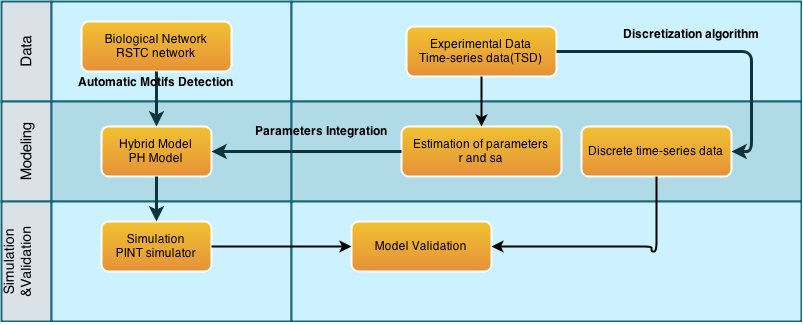
\includegraphics[width=6.5in]{images/workflow-2.png}
\caption{{\bf Workflow for integrating stochastic and temporal informations in large scale biological networks}} 
 \label{fig:workflow}
\end{figure*}

\begin{itemize}
 \item \textbf{Formalization of biological model.} Building a computational hybrid model  from biological network by automatic detection of known biological patterns.
 \item \textbf{Temporal parameters estimation.} Estimation of temporal parameters from times-series data to calibrate the model.
 \item \textbf{Integration of temporal parameters.} 
 \item \textbf{Discretization of times-series data.} Discretization of time series data to compare with discrete simulation results.
 \item \textbf{Simulation and validation.} Compare the results of simulation with the discretized times-series data.
\end{itemize}

\subsection{Data}

\subsubsection{Interaction network}
% \paragraph{The RSTC Network}
\label{ssec:RSTC}
The interactions of the biological system under study were represented in
 an RSTC network, which stands for  multi-layer receptor-signaling-transcription-cell state network, generated from the Pathway Interaction Database (PID).
In order to build this network, we selected a set of seed nodes related to the biological process studied.
The seed nodes for our case study were:  (1) \emph{E-cadherin}, which is a protein having $Ca$ binding domains and which plays an important role in cell adhesion;
(2) the $12$ significantly differentially expressed genes accross the $10$ time-points; and (3) the cell states of keratinocytes-differentiation and cell-cycle-arrest. 
The network was extracted automatically from the whole content of the NCI-PID database by using a subgraph algorithm to link the seed nodes \cite{guziolowski2012automatic}. 
In \pref{fig:network} we show the RSTC network obtained. 

\begin{definition}[RSTC Network] \label{def:RSTCDef}
A \emph{RSTC Network} $N$ is a couple $(V,E)$, where:
\begin{itemize}
\item $V =V_{T} \bigcup V_{I} $ is the finite set of \emph{nodes};
 with 
  $V_{T} = \{v_{1t},v_{2t}, \dots ,v_{n1t} \} $ the set of terminal nodes;
  $V_{I} = \{v_{1i},v_{2i}, \dots ,v_{n2i} \} $ the set of transient nodes.
\item $E = \{e_{1},e_{2}, \dots, e_{m} \}$ is the set of edges. $ E \subseteq (V_{T} \times V_{T}) \bigcup (V_{T} \times V_{I}) 
\bigcup (V_{I} \times V_{T})$
\end{itemize}
\end{definition}

In this definition, terminal nodes can be genes, proteins, complexes, cellular state, biological processes and positive condition. 
On the other side, transient nodes can be transcriptions, translocations, modifications and compounds. Edges are of different types.
We have activation (agent), inhibition, output, input and famillyMemberOf.

\begin{figure*}[!t]
 \centering
 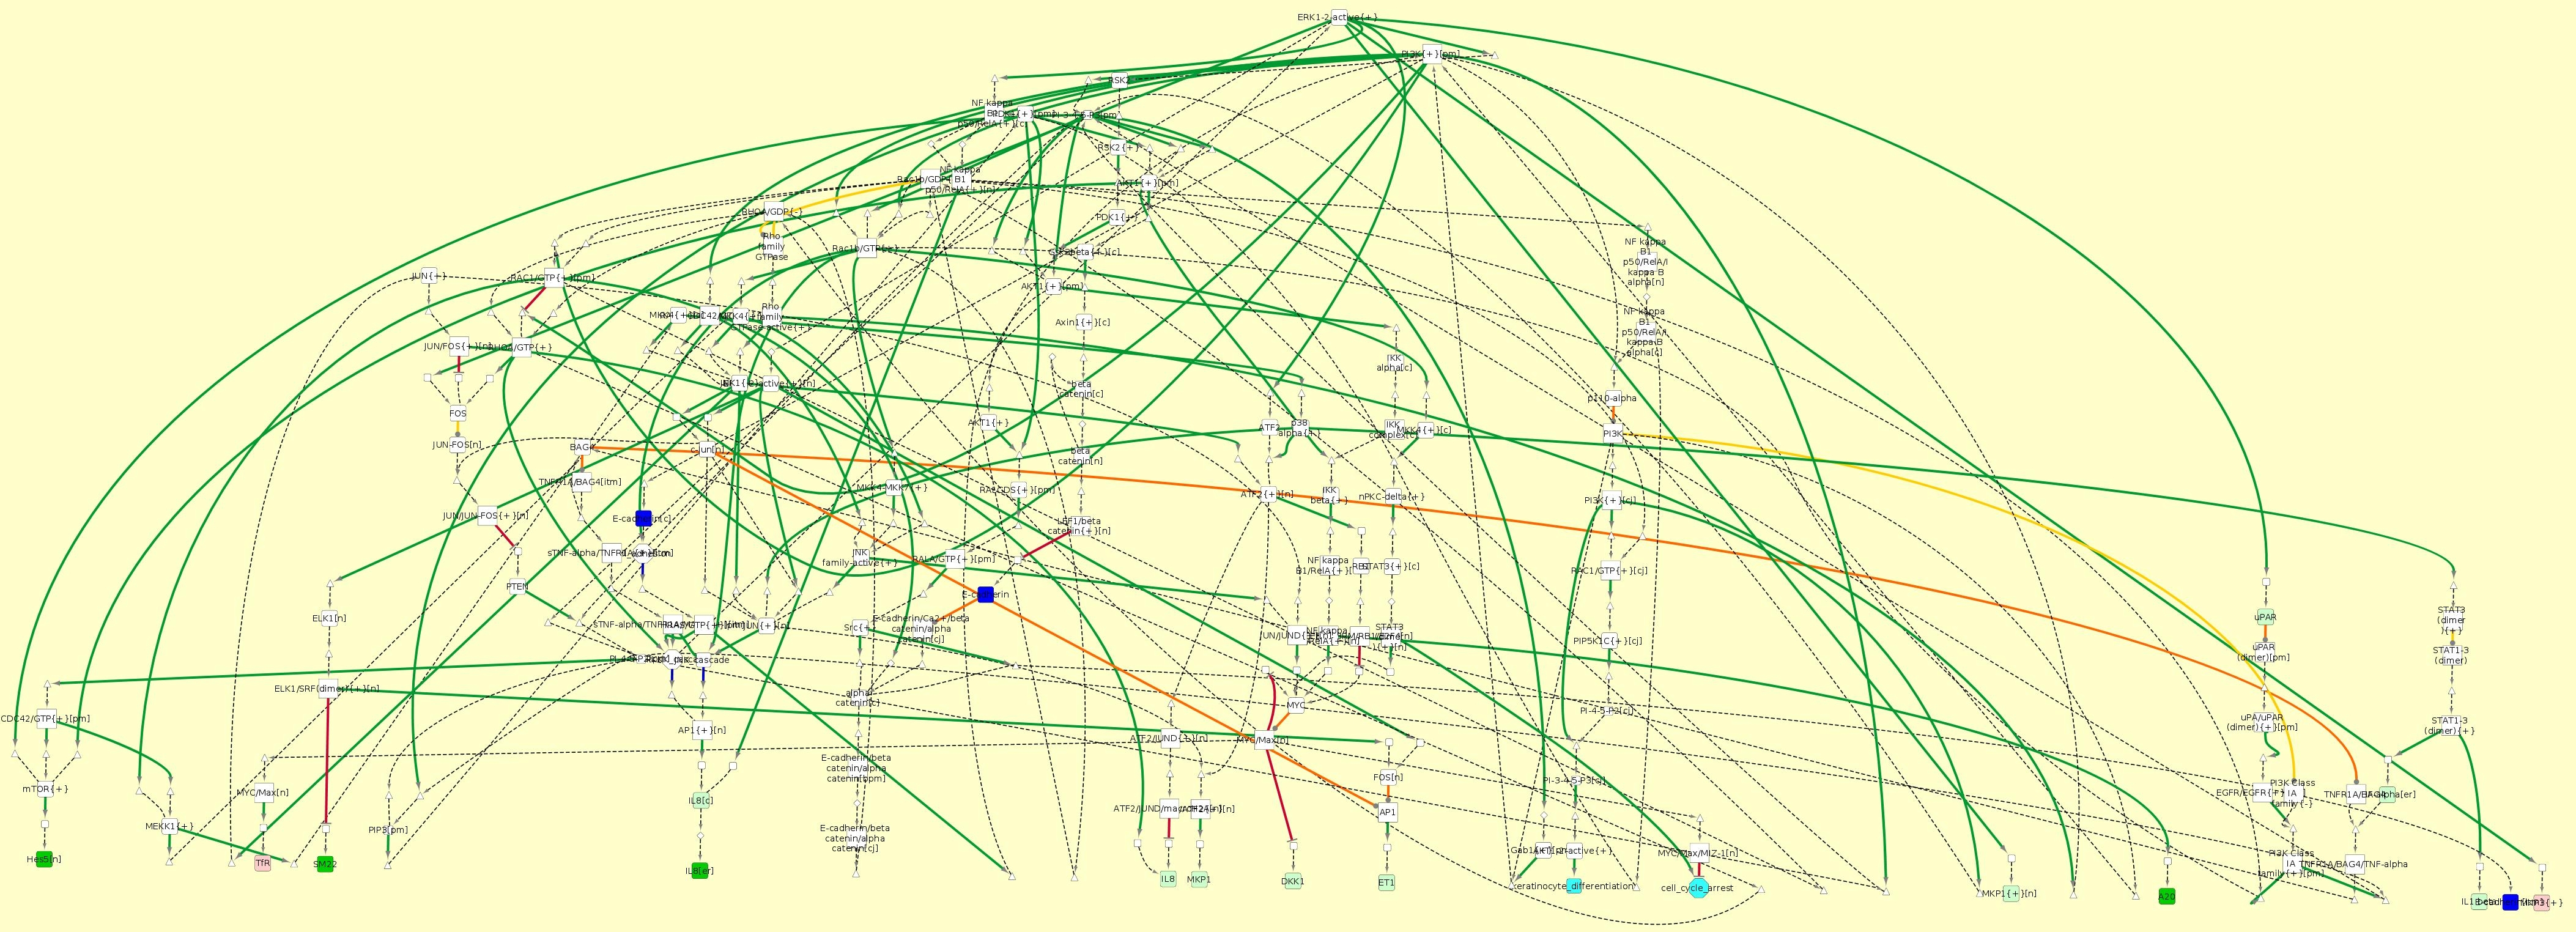
\includegraphics[width=6.5in]{images/net.jpg}
\caption{{\bf RSTC network. It is the interaction graph that describe the biological case study. It is composed of $293$ nodes and $375$ edges (interactions).
The set of nodes are composed of terminal nodes(proteins, complexes, genes, cellular state, biological processes and positive conditions) and of transient
nodes (transcriptions, compound, translocations, modifications and compounds). The set of edges are composed of interactions of type activation (agent), inhibition, output, 
input and famillyMemberOf}} 
 \label{fig:network}
\end{figure*}

%description des données
\subsubsection{Time-series microarray data description}
\label{SECTSD}
To illustrate our approach, we used the time-series microarray data from Calcium stimulated keratinocyte cells 
 measured at $10$ time-points. A $200$ transcripts were selected for their dynamic patterns,
that is, their fold expression with respect to the non-stimulated cell was significant in at least one time point. 
We included in our model a set of $12$ of the $200$ selected (see \pref{fig:tsd}), because we were able to retrieve the regulatory mechanisms upstream
these $12$ genes from public repositories of biochemical reactions.
The full dataset (data not shown) was produced by the German Cancer Research Center (DKFZ) and it's currently in the process
of getting published.  

\begin{figure}[!t]
\centering
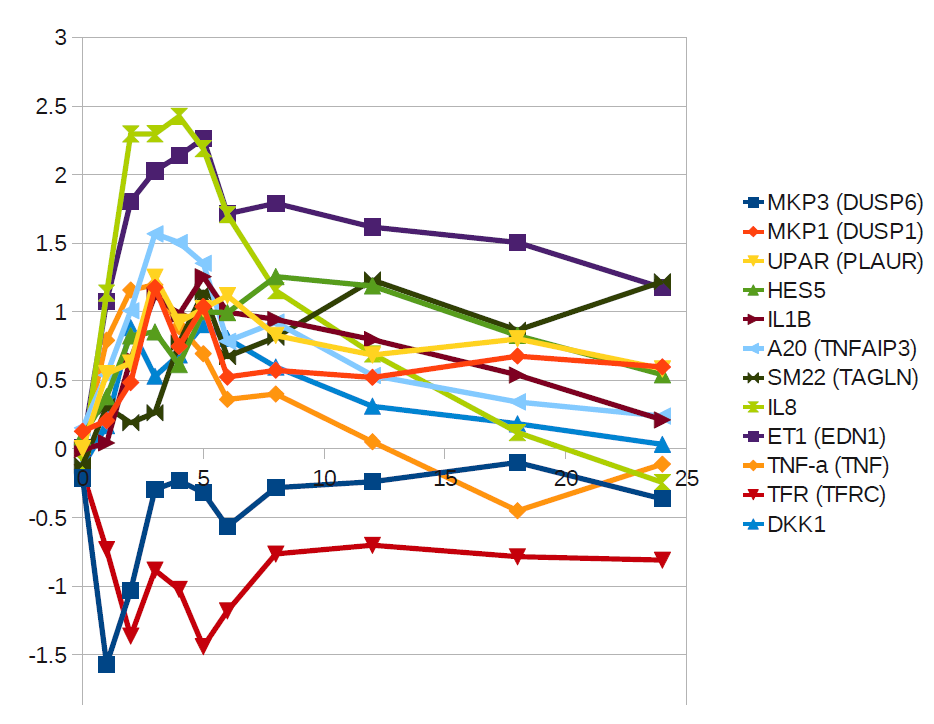
\includegraphics[width=2.5in]{images/12genes.png}
\caption{\bf Plot of $12$ selected genes}
\label{fig:tsd}
\end{figure}


\subsection{The Process  Hitting Framework}
\label{ssec:PH}

%We present here the Process Hitting framework \cite{PMR10-TCSB} which will enable us to model 
%biological network.

%\vspace{3mm}

Process Hitting (PH) gathers a finite number of concurrent processes grouped into a finite set of sorts.
A sort stands for a component of a biological system while a process, which belongs to a unique sort, stands
for one of its expression levels. At any time, exactly one process of each sort is present. A state of the 
PH corresponds to such a set of processes. We denote here a process by $a_i$ where $a$ 
is the sort and $i$ is the process identifier within the sort $a$.
The concurrent interactions between processes are defined by a set of \emph{actions}.
Actions describe the replacement of a process by another of the same sort conditioned by the presence 
of at most one other process in the current state. An action is denoted by $\PHfrappe{a_i}{b_j}{b_k}$, 
which is read as ``$a_i$ \emph{hits} $b_j$ to make it bounce to $b_k$'', where $a_i,b_j,b_k$ are 
processes of sorts $a$ and $b$, called respectively \emph{hitter}, \emph{target} and \emph{bounce} of 
the action.

\begin{definition}[Process Hitting] \label{def:PH}
A \emph{Process Hitting} is a triple $(\PHs,\PHl,\PHa)$, where:
\begin{itemize}
\item $\PHs = \{a,b,\dots\}$ is the finite set of \emph{sorts};
\item $\PHl = \prod_{a\in\PHs} \PHl_a$ is the set of states with $\PHl_a = \{a_0,\dots,a_{l_a}\}$
the finite set of \emph{processes} of sort $a\in\Sigma$ and $l_a$ a positive integer, with $a\neq b\Rightarrow \PHl_a \cap \PHl_b = \emptyset$;
\item $\PHa = \{ \PHfrappe{a_i}{b_j}{b_k} \in \PHl_a \times \PHl_b \times \PHl_b \mid (a,b) \in \PHs^2
  \wedge b_j\neq b_k \wedge a=b\Rightarrow a_i=b_j\}$ is the finite set of \emph{actions}.
\end{itemize}
\end{definition}

\noindent
Given a state $s\in \PHl$, the process of sort $a\in\PHs$ present in $s$ is denoted by $\PHget{s}{a}$.
An action $h=\PHfrappe{a_i}{b_j}{b_k} \in \PHa$ is \emph{playable} in $s \in L$ if and only if $\PHget{s}{a}=a_i$ and $\PHget{s}{b} = b_j$.
In such a case, $(s\play h)$ stands for the state resulting from the play of the action $h$ in $s$, with
$\PHget{(s\play h)}{b} = b_k$ and $\forall c \in \PHs, c \neq b, \PHget{(s\play h)}{c} = \PHget{s}{c}$.

\subsubsection{Modeling cooperation}

As described in \cite{PMR10-TCSB}, the cooperation between processes to make another process bounce can be
expressed in PH by building a \emph{cooperative sort}.
\pref{fig:runningPH} shows an example of a cooperative sort $ab$ between sorts $a$ and $b$,
defined with 4 processes (one for each sub-state of the presence of processes $a_1$ and $b_1$).
For the sake of clarity, processes of $ab$ are indexed using the sub-state they represent.
Hence, $ab_{01}$ represents the sub-state $\PHstate{a_0,b_1}$, and so on.
Each process of sort $a$ and $b$ hit $ab$, which makes it bounce to the process reflecting the status of the sorts $a$
and $b$ (e.g., $\PHfrappe{a_1}{ab_{00}}{ab_{10}}$ and $\PHfrappe{a_1}{ab_{01}}{ab_{11}}$).
Then, to represent the cooperation between processes $a_1$ and $b_1$,
the process $ab_{11}$ hits $c_1$ to make it bounce to $c_2$ instead of
independent hits from $a_1$ and $b_1$.
The same cooperative sort is used to make $a_0$ and $b_0$ cooperate to hit $c_1$ and make it bounce to $c_0$.
\subsubsection{Modeling synchronization}
%introdure la synchronization
Unlike cooperation sort which allow us to model the fact that two components cooperate to hit another component, we introduce
the notion of synchronization sort, which will implement another type of cooperation. If we refer to our example
\pref{fig:runningPH}, and asume that $ab$ is our \emph{synchronization sort} between sorts $a$ and $b$, defined with also 
4 processes. Then, component $c$ will be activated ($c_1$ bounce to $c_2$) if each one of $a$ and $b$ are also activated. So each 
one of this processes $ab_1$, $ab_2$, $ab_3$ can activate $c_1$. But to be desactived, we need both $a$ and $b$ to be desactived.
We will see later why it is important to introduce this new rule for the cooperation between componnets in our real case study.

Remember that PH was designed in order to take very large system analysis into account. Indeed, algorithm were developped on such a
process??? system so that it prevent for building the whole state graph which would be intractable when there are more than $10$ or 
$20$ components.

\begin{example}
\pref{fig:runningPH} represents a PH $(\PHs,\PHl,\PHa)$ with $\PHs = \{a,b,c,ab\}$, and:
\begin{align*}
\PHl_a &= \{a_0,a_1\},\\
\PHl_b &= \{b_0, b_1\},\\
\PHl_{ab} &= \{ab_{00}, ab_{01}, ab_{10}, ab_{11}\},&\\
\PHl_c &= \{c_0, c_1, c_2\}.
\end{align*}
This example models a Biological Regulatory Network (BRN) where the component $c$ has three qualitative levels, components $a$ and $b$ are Boolean and $ab$ is a cooperative sort.
In this BRN, $ab$ inhibits $c$ at level $2$ through the cooperative sort $ab$ (e.g. $\PHfrappe{ab_{00}}{c_2}{c_1}$, $\PHfrappe{ab_{00}}{c_1}{c_0}$) while $a$ and $b$ activate $c$  
through the cooperative sort $ab$ (e.g. $\PHfrappe{ab_{11}}{c_0}{c_1}$ $\PHfrappe{ab_{11}}{c_1}{c_2}$ ). Indeed, the reachability of $c_2$ and $c_0$ 
is conditioned by a cooperation of $a$ and $b$, as explained above.

\begin{figure}[!t]
%\centering
\begin{minipage}{0.3\linewidth}
\centering
\scalebox{0.7}{
\begin{tikzpicture}[grn]
\path[use as bounding box] (-0.2,-0.7) rectangle (3.5,0.7);
\node[inner sep=0] (a) at (1,2) {a};
\node[inner sep=0] (b) at (1,0) {b};
\node[inner sep=0] (c) at (3,1) {c};
\path[->]
  (b) edge node[elabel, above=-3pt] {$+$} (c)
  %(c) edge node[elabel, above=-5pt] {$1+$} (a)
  (a) edge node[elabel, above=-3pt] {$+$} (c);
\end{tikzpicture}
}
\end{minipage}
\begin{minipage}{0.7\linewidth}
\centering
\scalebox{0.7}{
\begin{tikzpicture}
\path[use as bounding box] (-2,-5.2) rectangle (7,0.7);

\TSort{(0,0)}{a}{2}{t}
\TSort{(0,-3.8)}{b}{2}{b}
\TSort{(4.5,-3)}{c}{3}{r}

\TSetTick{ab}{0}{00}
\TSetTick{ab}{1}{01}
\TSetTick{ab}{2}{10}
\TSetTick{ab}{3}{11}
\TSort{(-0.5,-2)}{ab}{4}{b}


\THit{a_1}{bend right}{ab_0}{.north}{ab_2}
\THit{a_1}{bend right}{ab_1}{.north}{ab_3}
\THit{a_0}{}{ab_2}{.north west}{ab_0}
\THit{a_0}{}{ab_3}{.north west}{ab_1}

\THit{b_0}{}{ab_1}{.south}{ab_0}
\THit{b_0}{}{ab_3}{.south}{ab_2}
\THit{b_1}{}{ab_0}{.south}{ab_1}
\THit{b_1}{}{ab_2}{.south}{ab_3}

\path[bounce, bend right=25]
\TBounce{ab_2}{}{ab_0}{.north east}
\TBounce{ab_3}{}{ab_1}{.north east}
;
\path[bounce, bend left=80, distance=30]
\TBounce{ab_0}{}{ab_2}{.north}
\TBounce{ab_1}{}{ab_3}{.north}
;
\path[bounce, bend right]
\TBounce{ab_0}{}{ab_1}{.west}
\TBounce{ab_2}{}{ab_3}{.west}
;
\path[bounce, bend left]
\TBounce{ab_3}{}{ab_2}{.east}
\TBounce{ab_1}{}{ab_0}{.east}
;

\THit{ab_3}{thick}{c_1}{.north west}{c_2}
\THit{ab_0}{thick,bend right=130, in=305, distance=140}{c_1}{.south east}{c_0}
\path[bounce, bend left=40]
\TBounce{c_1}{thick}{c_2}{.south west}
\TBounce{c_1}{thick}{c_0}{.north east}
;

\THit{ab_3}{thick}{c_0}{.north west}{c_1}
\THit{ab_0}{thick,bend right=130, in=305, distance=140}{c_2}{.south east}{c_1}
\path[bounce, bend left=40]
\TBounce{c_0}{thick}{c_1}{.south west}
\TBounce{c_2}{thick}{c_1}{.north east}
;


\end{tikzpicture}
}
\end{minipage}

\caption{\label{fig:modelingBRN}
(left)~Biological pattern example.
Nodes are components and edges are interactions
For instance, components $a$ and $b$ cooperate to activate $c$.
(right)~equivalent PH model. \label{fig:runningPH}
A PH example with four sorts: three components ($a$, $b$ and $c$) and a cooperative sort ($ab$).
Actions targeting processes of $c$ are in thick lines.
}
\end{figure}

\end{example}




%la traduction automatique des patterns d'un réseau
\subsection{Model construction(From RSTC to PH)}
%In this part we will describe how to go from rstc to ph model
In this work, we aim to model a biological  system according to his dynamic. For that, we choose to build a PH model from the biological model reprensented as  an RSTC network.

%why we made this choice?
In the following we present our automatic approach to generate a PH model from an RSTC network.


\subsubsection{Modeling the RSTC network as a PH model}

%In this section, we present the modelisation of biological network express with the biochemical reactions in PID. In the following, we will
%present how to transform biological pattern to the PH model. After that, we propose a way of estimating temporal and stochastic
%parameters for the process hitting model. This section will end by the generation of the PH code generation for the simulation.

%\paragraph{Modeling biological patterns to PH model}

%Here is the first and the most important part of this work. 
In order to model the RSTC network as a PH model we selected known biological regulatory patterns (atomic set of biological components and their interacting roles), represented 
as biochemical reactions in the RSTC network, and proposed their PH representation. 

%les ajouts pour les patterns 
We build an algorithm that will automatically browse the graph node by node and detect all patterns in the graph. More precisely, for each node(output node of the pattern) we will call a recursive procedure,
that will allow us to detect a minimal set of node(input node of the pattern) that has an direct influence on that node. This set of node plus the output node and the way there are linked are a pattern for us. 
The type of a pattern is determine by the type of the output node, the type of regulations come on that node and the type of input nodes of the pattern. So the algorithm that detect patterns return the pattern 
and its type to another procedure which one will traduce the pattern into the process hitting formalism. This transformation will take care of different case(cooperation, synchronization, simple activation, simple inhibition,...)



%nous avons des noeuds qui sont des composants du réseau, pour notre alogorithme(récursif) ils seront considérés comme noeuds initiaux et terminaux.
%nous avons des noeuds transitoires qui relient deux arrêtes entre elles afin d'indicquer la nature de l'interaction entre deux composants terminaux
%nous avons enfin les arrêtes qui relient les noeuds terminaux aux noeuds transitoires


%%%%algorithm of patterns detection in all the network

\begin{figure}[!t]
\begin{algorithmic}[1]
%\Procedure{patternDetection}{$Net,n$}\Comment{Given a node n, detect a set of minimal nodes that has a direct regulatory effect on n}
\REQUIRE $Net$
\ENSURE return all the patterns associated to the given network $Net$
\FORALL{ Node $n$ in $Net$ } 
\STATE $Pat$ = detectPattern($Net$, $n$)
\STATE patternInPHModel($out$,$Pat$)

\ENDFOR
%\STATE \textbf{return} $b$%\Comment{The gcd is b}
\end{algorithmic}
\caption{\bf Pattern detection in an RSTC Network}
\label{patternDetection}
\end{figure}


%%%%%algorithm for detect the pattern of a given node

\begin{figure}[!t]
\begin{algorithmic}[1]
%\Procedure{patternInPHModel}{$out,Pat$}\Comment{Write on the flux out the PH Model of a given pattern (Pat)}
\REQUIRE $Net$, $n$
\ENSURE Detect a pattern associated to a given node (n in this case)
%\WHILE{$r\not=0$}  %\Comment{We have the answer if r is 0}
\STATE 
\STATE 
\SWITCH {$n$}
 \CASE{TerminalNode} %\COMMENT{We compact many sub case of all terminal nodes}
   \STATE added node to the pattern
   \STATE numberPredecessor= $n$.getNumberOfPredecessor() \COMMENT{To get the number of predecessor of node $n$}
   \SWITCH{numberPredecessor}
   
   \CASE{1}
    \FORALL {in comming edge (n-m)}
    \STATE get the node $m$
    \SWITCH {$m$}
    \CASE {TerminalNode}
      \STATE added node to the pattern $Pat$
    \ENDCASE
    
    \CASE {TransientNode}
      \STATE detectPattern($Net$,$m$);
    \ENDCASE
    
    \ENDSWITCH
   \ENDFOR
      \STATE Set the code of pattern Pat
      \STATE return $Pat$
   \ENDCASE
   
     % \CASE {2}
  % \ENDCASE
  % \DEFAULT
  %  \STATE \RETURN ERROR CODE \COMMENT{We can't treat this case}
  % \ENDDEFAULT
   \ENDSWITCH
\ENDCASE
   
   \CASE{TransientNode} %\COMMENT{We compact many sub case of all terminal nodes}
   %\STATE added node to the pattern
   \STATE numberPredecessor= $n$.getNumberOfPredecessor() \COMMENT{To get the number of predecessor of node $n$}
   \SWITCH{numberPredecessor}
   
   \CASE{1}
    \FORALL {in comming edge (n-m)}
    \STATE get the node $m$
    \SWITCH {$m$}
    \CASE {TerminalNode}
      \STATE added node to the pattern $Pat$
    \ENDCASE
    
    \CASE {TransientNode}
      \STATE detectPattern($Net$,$m$);
    \ENDCASE
    
    \ENDSWITCH
   \ENDFOR
      \STATE Set the code of pattern Pat
      \STATE return $Pat$
   \ENDCASE
   
  % \CASE {2}
  % \ENDCASE
  % \DEFAULT
  %  \STATE \RETURN ERROR CODE \COMMENT{We can't treat this case}
  % \ENDDEFAULT
   \ENDSWITCH
\ENDCASE
%\CASELINE {2}
%  \STATE Good-bye
%\DEFAULT
%  \STATE Again ?
%\ENDDEFAULT
\ENDSWITCH
%\ENDWHILE\label{euclidendwhile}
\end{algorithmic}
\caption{\bf Detection of Pattern associated to the node n} \label{PatternDetectionNode}
\end{figure}



%%%%%algorithm for write the pattern in PH model

\begin{figure}[!t]
\begin{algorithmic}[1]
%\Procedure{patternInPHModel}{$out,Pat$}\Comment{Write on the flux out the PH Model of a given pattern (Pat)}
\REQUIRE $out$, $Pat$ \COMMENT{ Pat is The pattern to be translate into the PH Model, out is the output file}
\ENSURE The correspondant PH Model of the given pattern Pat will write into the file $out$
%\WHILE{$r\not=0$}  %\Comment{We have the answer if r is 0}
\STATE $nocp$ = $Pat$.getNumberOfComponents() \COMMENT{Number of the components of the pattern $Pat$}
\STATE 
\SWITCH {$nocp$}
 \CASE {2}
  \SWITCH {$type$}
 \CASE {A}
   \STATE out.write("activation")
   \STATE out.write("")
        
\ENDCASE
\CASELINE {I}
  \STATE out.write("inhibition")
  \STATE 
\DEFAULT
 \STATE out.write("unknow pattern")
 \ENDDEFAULT
\ENDSWITCH
   
   
\ENDCASE

\CASE {3}
  \SWITCH {$type$}
 \CASE {C}
   \STATE out.write("cooperation")
        
\ENDCASE
\CASELINE {S}
  \STATE out.write("synchronization")
\DEFAULT
 \STATE out.write("unknow pattern")
 \ENDDEFAULT
\ENDSWITCH
   
   
\ENDCASE
%\CASELINE {2}
%  \STATE Good-bye
%\DEFAULT
%  \STATE Again ?
%\ENDDEFAULT
\ENDSWITCH
%\ENDWHILE\label{euclidendwhile}
\end{algorithmic}
\caption{\bf Pattern in PH Model} \label{PHModel}
\end{figure}


% les détails sur comment les patterns sont choisis 
For example a molecule $a$ that cooperates with a molecule $b$ to activate a molecule $c$ \pref{fig:runningPH} (top), is a regulatory pattern because it is a protein-complex biochemical reaction that appears recurrent times.  
We model this pattern by four sorts \pref{fig:runningPH} (bottom) $a$, $b$, $c$ and $ab$. Sorts $a$, $b$ and $c$
represent components $a$, $b$ and $c$. We introduce the cooperative sort $ab$ to characterize constraints on components $a$ and $b$.
In our RSTC network, we found $11$(to be precise...) regulatory patterns (see Appendix \ref{table_patterns}). 

\begin{table}[!t]
\renewcommand{\arraystretch}{1.3}
\caption{Examples of patterns}
\label{table_patterns}
\centering
\begin{tabular}{c||c}
\hline
\bfseries Biological Patterns

&

\bfseries PH Transformations\\ 
\hline\hline
\begin{tikzpicture}
\node[scale=0.5] (sa1) at (0,0){\begin{tikzpicture}[auto]
\path[use as bounding box] (-0.7,-0.3) rectangle (2.5,2);

\node[qgre] (a) at (0,1) {a};
\node[mod] (i) at (1,1) {i};
\node[qgre] (b) at (2,1) {b};
\node[es] (d) at (1,2) {Simple activation};

\path
 (a) edge[act] (i)
 (i) edge[st]  (b);
\end{tikzpicture}};
\end{tikzpicture}

&


\begin{tikzpicture}
%\exphpatact
\node[scale=0.5] (sa) at (0,0) {\begin{tikzpicture}
\path[use as bounding box] (-0.5,-0.5) rectangle (2.5,2.5);

\TSort{(0,0.5)}{a}{2}{l}
\TSort{(2,0.5)}{b}{2}{l}
%\TSort{(6,1)}{z}{3}{r}

\THit{a_1}{}{b_0}{.west}{b_1}
\THit{a_0}{}{b_1}{.west}{b_0}
%\THit{a_0}{out=250,in=200,selfhit}{a_0}{.west}{a_1}

\path[bounce,bend left]
\TBounce{b_0}{}{b_1}{.south}
\TBounce{b_1}{bend right}{b_0}{.north}
%\TBounce{a_0}{}{a_1}{.south}
;
\end{tikzpicture}};
\end{tikzpicture}\\ 
\hline\hline

\begin{tikzpicture}
\node[scale=0.5] (si1) at (0,0){\begin{tikzpicture}[auto]
\path[use as bounding box] (-0.7,-0.3) rectangle (2.5,2);

\node[qgre] (a) at (0,1) {a};
\node[mod] (i) at (1,1) {i};
\node[qgre] (b) at (2,1) {b};
\node[es] (d) at (1,2) {Simple inhibition};
\path
 (a) edge[inh] (i)
 (i) edge[st]  (b);
 \end{tikzpicture}};
\end{tikzpicture}

&

\begin{tikzpicture}
%\exphpatact
\node[scale=0.5] (sa) at (0,0) {\begin{tikzpicture}
\path[use as bounding box] (-0.5,-0.5) rectangle (2.5,2.5);

\TSort{(0,0.5)}{a}{2}{l}
\TSort{(2,0.5)}{b}{2}{l}
%\TSort{(6,1)}{z}{3}{r}

\THit{a_1}{}{b_1}{.west}{b_0}
\THit{a_0}{}{b_0}{.west}{b_1}
%\THit{a_0}{out=250,in=200,selfhit}{a_0}{.west}{a_1}

\path[bounce,bend left]
\TBounce{b_1}{bend right}{b_0}{.north}
\TBounce{b_0}{}{b_1}{.south}
%\TBounce{a_0}{}{a_1}{.south}
;
\end{tikzpicture}};
\end{tikzpicture}\\ 
\hline\hline

\begin{tikzpicture}
\node[scale=0.5] (sai1) at (0,0){\begin{tikzpicture}[auto]
\path[use as bounding box] (-0.7,-0.3) rectangle (2.5,3);
\node[qgre] (a) at (0,2) {a};
\node[mod] (i) at (1,1) {i};
\node[qgre] (b) at (0,0) {b};
\node[qgre] (c) at (2,1) {c};
\node[es] (d) at (1,3) {activation or inhibition};

\path
 (a) edge[act] (i)
 (b) edge[inh] (i)
 (i) edge[st]  (c);
\end{tikzpicture}};
\end{tikzpicture}


&

\begin{tikzpicture}
%\exphpatact
\node[scale=0.5] (sai) at (0,0) {\begin{tikzpicture}
\path[use as bounding box] (-0.5,-0.5) rectangle (2.5,5.5);

\TSort{(0,0)}{a}{2}{l}
\TSort{(0,3)}{b}{2}{l}
\TSort{(2,1)}{c}{2}{r}

\THit{a_1}{}{c_0}{.west}{c_1}
\THit{a_0}{}{c_1}{.west}{c_0}
\THit{b_1}{}{c_1}{.west}{c_0}
\THit{b_0}{}{c_0}{.west}{c_1}

%\THit{a_0}{out=250,in=200,selfhit}{a_0}{.west}{a_1}

\path[bounce,bend left]
\TBounce{c_1}{bend right}{c_0}{.north}
\TBounce{c_0}{}{c_1}{.south}
%\TBounce{a_0}{}{a_1}{.south}
;
\end{tikzpicture}};
\end{tikzpicture} \\
\hline
\end{tabular}
\end{table}




%\subsubsection{Integrating parameters from  time-series gene expression data}

% the goal of this section (expliquer comment et pourquoi nous allons partir des séries temporelles pour estimer les rates des actions
%This section will present how we introduce temporal feature into a formal model. The temporal informations come from TSD and we want to emphases the notion of chronometric
%or delay. 





\subsubsection{Estimating the parameters for the PH-simulation from time-series gene expression data}

%peut etre penser à faire un schéma

The simulation of the execution of the PH actions is done stochastically.  Therefore, we need to relate each action with temporal 
and stochastic parameters, introduced into the PH framework to achieve dynamic refinement \cite{PMR10-TCSB}. 
This is an important aspect of the modeling when taking into account the temporal and stochastic dimensions of 
biological reactions by performing simulations. 
On the one hand, we consider the probability of a reaction to occur, and on the other hand, we 
consider stochastic parameters in the aim at observing an expected behavior. 
In the PH framework, to play an action we need two essential parameters: the rate $r$ or the temporal parameter because $t=r^{-1}$ if we assume that $t$ is the average time of playing an action
and the stochasticity absorption $sa$. These two parameters will be estimated according to the expression profile of time-series data of the experiment
described in Section \ref{SECTSD}. 


%To avoid over fitting in the estimation of these parameters, we propose that each component of the PH, representing a measured gene in the network,  will take the estimated values of the parameters of its respective cluster in the experimental data.



%\begin{enumerate}
% \item The first step is to cluster the data set. The goal of the clustering process is to partition genes into groups such that the 
% profiles contained in the same group (cluster) are similar to each other and as different as possible from the profiles assigned to the other
% clusters. The particularity here is to choose the best clustering criteria.
% \item For each cluster obtained in the previous step, estimate the value of $r$ and $sa$ associated to the cluster.
% \item For each component of the PH model associated to the measured gene, determine its cluster, and assign it $r$ and $sa$, the previously  estimated  parameters.
%\end{enumerate}

%In our time-series data the components of the PH which need to be associated specific parameters (step 3) are the $12$ genes present in our RSTC network.

\begin{figure}[!t]
\centering

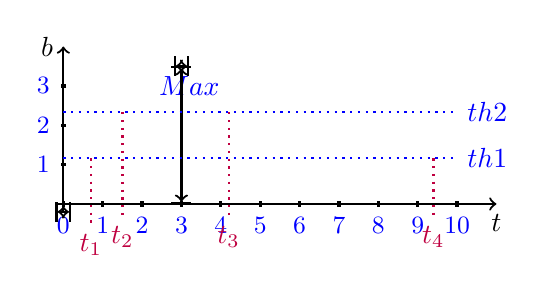
\begin{tikzpicture}[scale = 0.5]
       
    
	      \draw[thick, ->] (-.2,0)--(11,0) node[below]{$t$};
	      \foreach \t in {0,1,2,3,4,...,10}
	      \draw[very thick] (\t,2pt)--(\t,-2pt) node[below,blue]{\small\t};

	      \draw[thick, ->] (0,-.2)--(0,4) node[left]{$b$};
	      \foreach \y in {1,2,3}
	      \draw[very thick] (2pt,\y)--(-2pt,\y) node[left,blue]{\small\y};
      
	      \draw[thick] plot[mark=ball,mark size=1pt] file {illustration.txt};
    
	      %\pause
	      \draw[thick,|<->|] (2.8,3.5) -- (3.2,3.5) node[below,blue]{$Max$};
	      \draw[thick,|<->|] (-.2,-.2) -- (.2,-.2) node[below,blue]{};
	      %\pause
	      \draw[thick,|<->|] (3,0) -- (3,3.5);
	      %\pause
	      \draw[thick,dotted,blue] (0,1.16) -- (10,1.16) node[right]{$th1$}; 
	      \draw[thick,dotted,blue] (0,2.33) -- (10,2.33) node[right]{$th2$}; 
	      %\pause
	      \draw[thick,dotted,purple] (0.7,1.16) -- (0.7,-.5) node[below]{$t_{1}$};
	      %\pause
	      \draw[thick,dotted,purple] (1.5,2.33) -- (1.5,-.3) node[below]{$t_{2}$};
	      %\pause
	      \draw[thick,dotted,purple] (4.2,2.33) -- (4.2,-.3) node[below]{$t_{3}$};
	      %\pause
	      \draw[thick,dotted,purple] (9.4,1.16) -- (9.4,-.3) node[below]{$t_{4}$};

           \end{tikzpicture}
	    

\caption{Illustration of estimation of temporal parameters:$r_{i}=\frac{1}{t_{i}-t_{i-1}}$. $Max$ represents the maximum expression. $Min$ represents the minimum 
expression. In this example is $0$ the minimum level. $th1$ and $th2$ represent respectively the first and the second threshold.}
\label{fig:estimationParameter}
\end{figure}

\subsubsection{From data to action parameters}

%l'Introduction des données temporelles n'était pas automatique, de plus on ne savait pas le faire des données des séries temporelles.
%Before this work, it were not possible to infer temporal parameters from TSD and integrate them automatically into a model build in to the process hitting formalism.
%It's now possible. For components that we have measured, we know how to estimate and integrate parameters. For others that we don't have measured, we can give default parameters.
For the model, components, which have a measurement in the Time Series Data we estimate and integrate $r$ and $sa$ parameters in the PH model. For others, we assign default 
parameters. In other to estimate $r$ and $sa$ we ...


%discretisation des données
\subsubsection{Discretization of times-series data}

Because PH simulation is discrete we need to discretize continuous experimental data so we can compare our simulation outputs.
The goal of this method was to better determine, according to the gene expression level, when  a given molecule is activated or inhibited.
To do this, we introduced the new analog concept of Significant Increase or Decrease to characterize the fact that a level of a molecule 
increases or decreases when crossing a threshold of significance; we limited the possible expression levels for a molecule to
$\{0, 1, 2\}$. We made this choice because when we look our time-series data (see \pref{fig:tsd}), we can clearly observe a high level of
activity between $0h$ and $5h$ and a slow level of activity between $5h$ and $10h$ on the other hand. The goal of the discretization method is to capture these
two activation times. For each time-series, we introduce two thresholds \emph{th1} and \emph{th2} as in \pref{fig:estimationParameter}. The value of this two
thresholds is compute as follows $\emph{th1}=\frac{1}{3}(MaxLevel-MinLevel)$ and $\emph{th2}=\frac{2}{3}(MaxLevel-MinLevel)$. Therefore, all
of the expression level in the range $[0-th1]$ will have level $0$, all those in the range $[th1-th2]$ will have level $1$ and the last group will
have level $2$. In  this way we can automatically determine the differents levels of expression of the TSD. 
%illustration des résultats de la méthode de discrétisation
To illustrate the result of our discretization algorithm we plot in \pref{fig:illustrationDiscretisation} the expression 
of $9$ seleted genes from the times-series data with their respective discrete plots. 
%On the discrete plot, one can clearly differentiate when a molecule is active or not, which is of extreme importance 
%swhen modeling these steps in the PH framework if we would like to have coherent simulation results.

\begin{figure*}[!t]
 \centering
 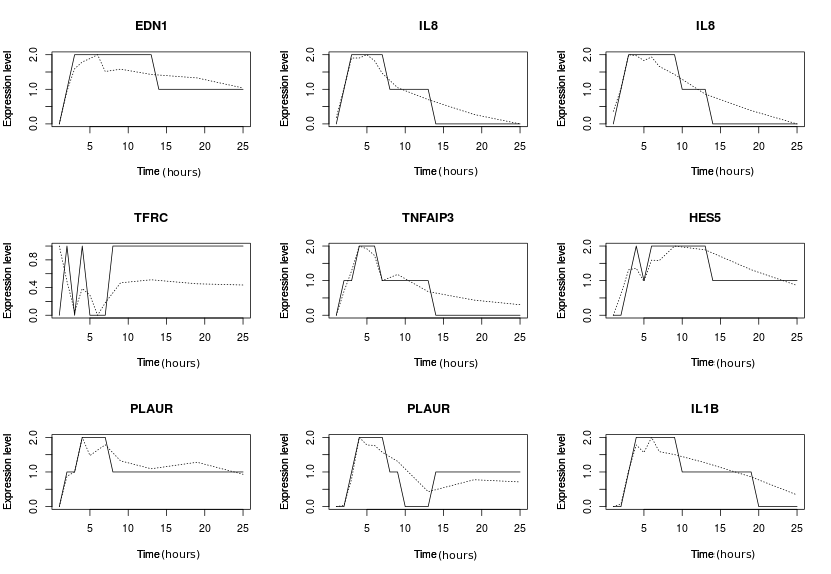
\includegraphics[width=6.5in,height=3.5in]{images/ResultDiscretization.png}
 % IllustrationDiscretisation.png: 831x574 pixel, 72dpi, 29.32x20.25 cm, bb=0 0 831 574
 \caption{Illustration of discretization of experimental data. Continous lines are descrite data, dashed lines are continuous data}
 \label{fig:illustrationDiscretisation}
\end{figure*}

  


\subsection{Simulation: Initials conditions}
%we give the initial condition for the simulation
To run the simulation we need to set initial conditions for the components of our network. Because the components of the network are grouped into 
layers, the initial conditions will be the same in the different layers. In the following we will present the initial conditions that we have chosen for the different 
components.

\begin{itemize}
 \item \textbf{Receptor layer: E-cadherin.} We choose the  pulse signal for the input node E-cadherin, that will be active for a duration of average $x$ units times. We made this 
 choice to take into account the average time of calcium stimuli effect.
 \item \textbf{Signaling layer: signaling proteins.} At this layer, the components will be activated and inhibited according to the same rate and the same stochasticity absorption factor.
 The values of these parameters where selected by considering the time of signal transduction from the entry node (E-cadherin) to the output node (genes).[imposing reachability
 constraints from entry node Ecad].
 \item \textbf{Transcription layer: transcription factors.} At this stage, the signal will come from signaling proteins for activation. But for the inhibition, in addition 
 of the signal come from signaling proteins, we introduce an auto-inhibition which will represented a degradation of the transcription factor.
 \item \textbf{Cell-state: genes and cellular  process.} The genes will be activited or inhibited according to the estimated values from time-series data.
\end{itemize}

We summarize the initial conditions of our simulation in \pref{fig:initialCondition} were we can clearly see the initial values choose at each layer for our model.

\begin{figure}[!t]
 \centering
 \scalebox{0.45}{
  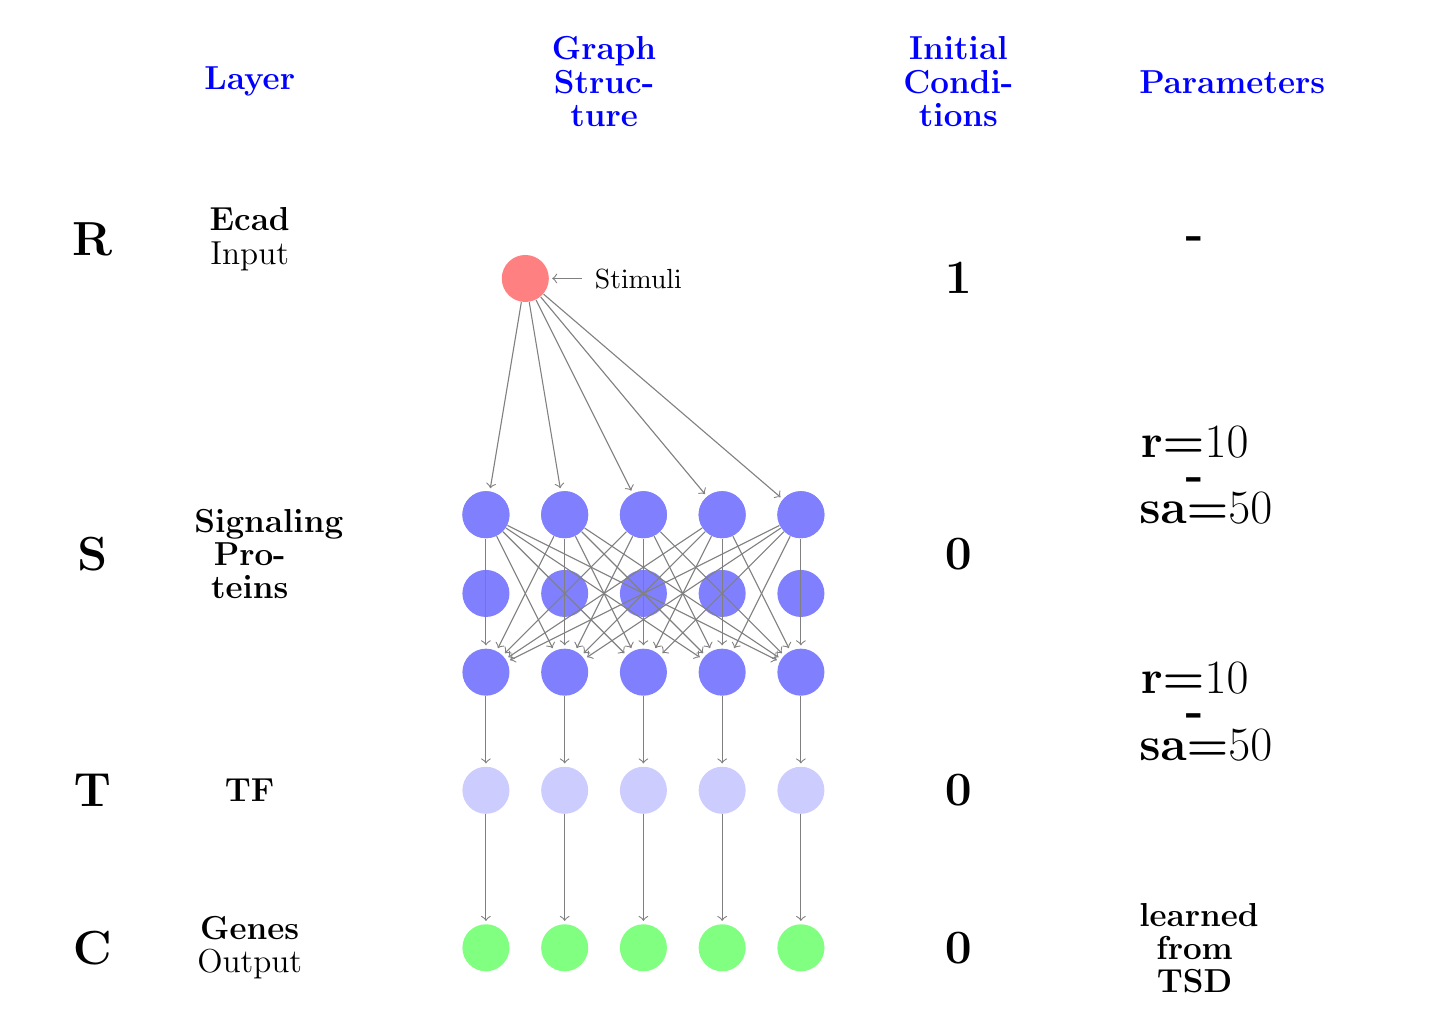
\begin{tikzpicture}[shorten >=1pt,->,draw=black!50, node distance=\layersep]
    \tikzstyle{every pin edge}=[<-,shorten <=1pt]
    \tikzstyle{neuron}=[circle,fill=black!25,minimum size=17pt,inner sep=0pt]
    \tikzstyle{input neuron}=[neuron, fill=green!50];
    \tikzstyle{output neuron}=[neuron, fill=red!50];
    \tikzstyle{hidden neuron}=[neuron, fill=blue!50];
    \tikzstyle{transfact neuron}=[neuron, fill=blue!20];
    \tikzstyle{annot} = [text width=4em, text centered]

    % Draw the input layer nodes
    \foreach \name / \x in {1,...,5}
    % This is the same as writing \foreach \name / \y in {1/1,2/2,3/3,4/4}
       % \node[input neuron, pin=left:Output \#\y] (I-\name) at (0,-\y) {};
         \node[input neuron] (I-\name) at (\x-7,-4) {};

     % Draw the transcription factor layer node
    \foreach \name / \x in {1,...,5}
    % This is the same as writing \foreach \name / \y in {1/1,2/2,3/3,4/4}
       % \node[input neuron, pin=left:Output \#\y] (I-\name) at (0,-\y) {};
         \node[transfact neuron] (TF-\name) at (\x-7,-2) {};
     
     
     % Draw the hidden layer nodes
    \foreach \name / \x in {1,...,5}
        \path[yshift=0.5cm]
           % node[hidden neuron] (H-\name) at (\layersep,-\y cm) {};
             node[hidden neuron] (H-\name) at (\x-7 , \layersep) {};
             
    
    % Draw the hidden layer nodes
    \foreach \name / \x in {1,...,5}
        \path[yshift=0.5cm]
           % node[hidden neuron] (H-\name) at (\layersep,-\y cm) {};
             node[hidden neuron] (H1-\name) at (\x-7 ,1) {};
             
     % Draw the hidden layer nodes 1
    \foreach \name / \x in {1,...,5}
        \path[yshift=0.5cm]
           % node[hidden neuron] (H-\name) at (\layersep,-\y cm) {};
             node[hidden neuron] (H2-\name) at (\x-7 ,0) {};
             
     % Draw the hidden layer nodes 2
    \foreach \name / \x in {1,...,5}
        \path[yshift=0.5cm]
           % node[hidden neuron] (H-\name) at (\layersep,-\y cm) {};
             node[hidden neuron] (H3-\name) at (\x-7 ,-1) {};
             
    % Draw the output layer node
     \node[output neuron,pin={[pin edge={<-}]right:Stimuli}] (O) at (2.5-8,4.5) {};
     
     
   %connect nodes   

    % Connect every node in the input layer with every node in the
    % hidden layer.
    \foreach \source in {1,...,5}
        \foreach \dest in {1,...,5}
            \path (H-\dest) edge (H3-\source);

    % Connect every node in the hidden layer with the output layer
    \foreach \source in {1,...,5}
        \path (O) edge (H-\source) ;
        
   %connect sp to tf
   \foreach \source in {1,...,5}
    \path (H3-\source) edge (TF-\source);
        
    %connect TF with Genes
    
    \foreach \source in {1,...,5}
     \path (TF-\source) edge (I-\source);
     
      %titre du graphe
    \node[annot] (graphTitle) at (2.5-7,7) {\textcolor{blue}{\large \textbf{Graph Structure}}};

    % Annotate the layers
    \node[annot] (layerTitle) at (-9,7) {\textcolor{blue}{\large \textbf{Layer}}};
    \node[annot, node distance=1cm] (couchesp) at (-9,1) {\large \textbf{Signaling Proteins} };
    \node[annot] (coucheFT) at (-9,-2) {\large \textbf{TF} };
    \node[annot] (coucheGene) at (-9,-4) {\large \textbf{Genes} Output };
    \node[annot] (noeudEntre) at (-9,5) {\large \textbf{Ecad} Input };
    
    %noeud pour ajouter le R S T C 
    \node[annot] (R) at (-11,5) {\textcolor{black}{\textbf{\LARGE R}}};
    \node[annot] (S) at (-11,1) {\textcolor{black}{\textbf{\LARGE S}}};
    \node[annot] (T) at (-11,-2) {\textcolor{black}{\textbf{\LARGE T}}};
    \node[annot] (C) at (-11,-4) {\textcolor{black}{\textbf{\LARGE C}}};
    \node[annot] (test) at (5,-4) {\textcolor{black}{\textbf{}}};
    
    %noeud pour les règles de modélisation
    \node[annot] (icTitle) at (0,7) {\textcolor{blue}{\textbf{\large Initial Conditions}}};
    \node[annot] (RMi) at (0,4.5) {\textcolor{black}{\textbf{\LARGE 1}}};
    \node[annot] (SMi) at (0,1) {\textcolor{black}{\textbf{\LARGE 0}}};
    \node[annot] (TMi) at (0,-2) {\textcolor{black}{\textbf{\LARGE 0}}};
    \node[annot] (CMi) at (0,-4) {\textcolor{black}{\textbf{\LARGE 0}}};
    %\node[annot] (P) at (5,-4) {\textcolor{black}{\huge \textbf{}}};
    
    %noeuds pour les hypothèses de modélisation 
    \node[annot] (parameterTitle) at (3,7) {\textcolor{blue}{\textbf{\large Parameters}}};   %text width=3cm
    \node[annot] (RH) at (3,5) {\textcolor{black}{\textbf{\LARGE -}}};
    \node[annot] (SH) at (3,2) {\textcolor{black}{\small \textbf{\LARGE r=$10$ - sa=$50$}}};
    \node[annot] (TH) at (3,-1) {\textcolor{black}{\small \textbf{\LARGE r=$10$ - sa=$50$}}};
    \node[annot] (CH) at (3,-4) {\textcolor{black}{\small \textbf{\large learned from TSD}}};
    %\node[annot] (test) at (5,-4) {\textcolor{black}{\huge \textbf{}}};
    
    %noeuds de repères pour les sous-graphs
    
    \node[annot] (R1) at (-4.7,\layersep) {};
    \node[annot] (R2) at (-4.7,1) {};
    \node[annot] (R3) at (-6.8,-1) {};
    \node[annot] (R4) at (-6.5,-4) {};
    \node[annot] (R5) at (-6.5,\layersep) {};
    
   
     
\end{tikzpicture}
}

 
 \caption{RSTC network structure and initial conditions assigned to each node in the layer}
 \label{fig:initialCondition}
\end{figure}



\section{Results}

\subsection{From PID to PH: An automatic generation of PH code of the network}
%give statistics

To simulate of the model we generated a PINT code to be simulated by the PINT simulator \footnote{Available at \url{http://process.hitting.free.fr}}. 
PINT implements static analyses for computing dynamical properties on very large-scale Automata Networks.
For the PINT code generation we use two procedures as described in the method section. The first procedure that detects the patterns and its code; the second 
procedure that generates the PINT code by taking in consideration the type of the pattern to better refine the dynamic of the system from a structural point of view.
This refinement is done by introducing the synchronization sort  which is a generalization of the cooperation sort. This allows  to avoid artificial oscillations
in the dynamics of the components of the system.


%procedure take a in parameter a pattern with its code from the procedure of detection of patterns. Afater taking 
%the pattern, the procedure will write the correct code associate to the current pattern. 
%list all the selected patterns in the biological reaction into a file. In this file, each line contains the 
%name of the nodes belonging to the current reaction and the reaction type number. The list was then parsed, line by line and, 
%after renaming the nodes using numbers (for readability and in conformity with the PINT language syntax) the corresponding PINT code
%for the PH process equivalent to each reaction was generated. This was implemented in a Java code.


\subsection{Simulation}
%present the simulation results
%In this section we will present the results of the simulations of the model. It will be present in two 
%main sub sections. In the first, we will present the result of simulation of model without the inclusion 
%of the synchronization gate and in the second we will present result with synchronization gate. Both results
%present common characteristics and show us the coherence of our approach of modelization. The common characteristics
%are the following:

We simulated the model with and without the inclusion of the synchronization sort. In the following, we present the results of 
the simulation.

\subsubsection{Without the introduction of synchronization sort}
One can easily notice in \pref{fig:rwos} the occurence of oscillations. This is not the expected behavior from the biological system
but it is coherent with the choice of the modelling and the way the simulator works as explained in \ref{sssec:synchronization}: cooperation
sorts are used to model multiple regulators of a common target
where this is clearly identifiable. In other cases we left the components act independently.
It is important to notice that the intensity of the oscillation is linked with 
the size of the concurrence, i.e. the number of predecessors that a node in the network has.
Despite the presence of the oscillations, the model reproduces expected dynamical behavoirs  namely
the dynamic of components, the signal transduction and takes into account the stochastic and time aspect of the model.

\begin{figure*}[!t]
\centering
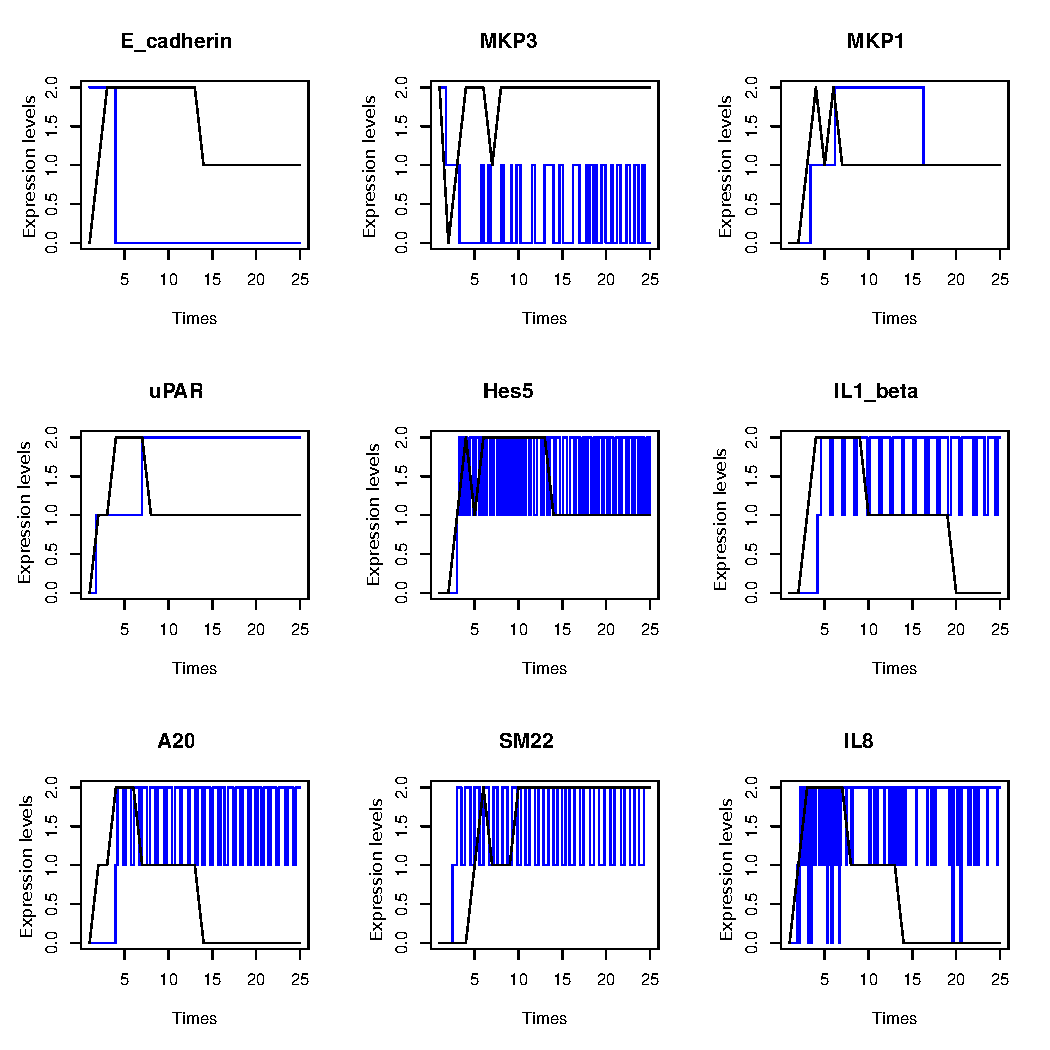
\includegraphics[width=6.5in,height=3.5in]{images/resultWOS.pdf}
\caption{\bf Results of simulations without introducing the synchronization sort. In black line the expected behaviours
come from the discretization of time-series data. In Blue line the simulation behavior.}
\label{fig:rwos}
\end{figure*}
\subsubsection{With the introduction of synchronization sort}

From \pref{fig:rws} we can see that the introduction of the synchronization sort significatively reduces the 
impact of concurrence by the introduction of the synchronization. The result shows  a 
clear elimination of the previously observed oscillation in \pref{fig:rwos}. One can see that the expression levels of genes \emph{uPAR}, \emph{MKP1},
\emph{IL1 beta} are well reproduced, while \emph{Hes5} and \emph{IL8} are not activated. This result can be observed when the activation
signal has not been able to propagate through the network due to the non determinism  and concurrency.


\begin{figure*}[!t]
\centering
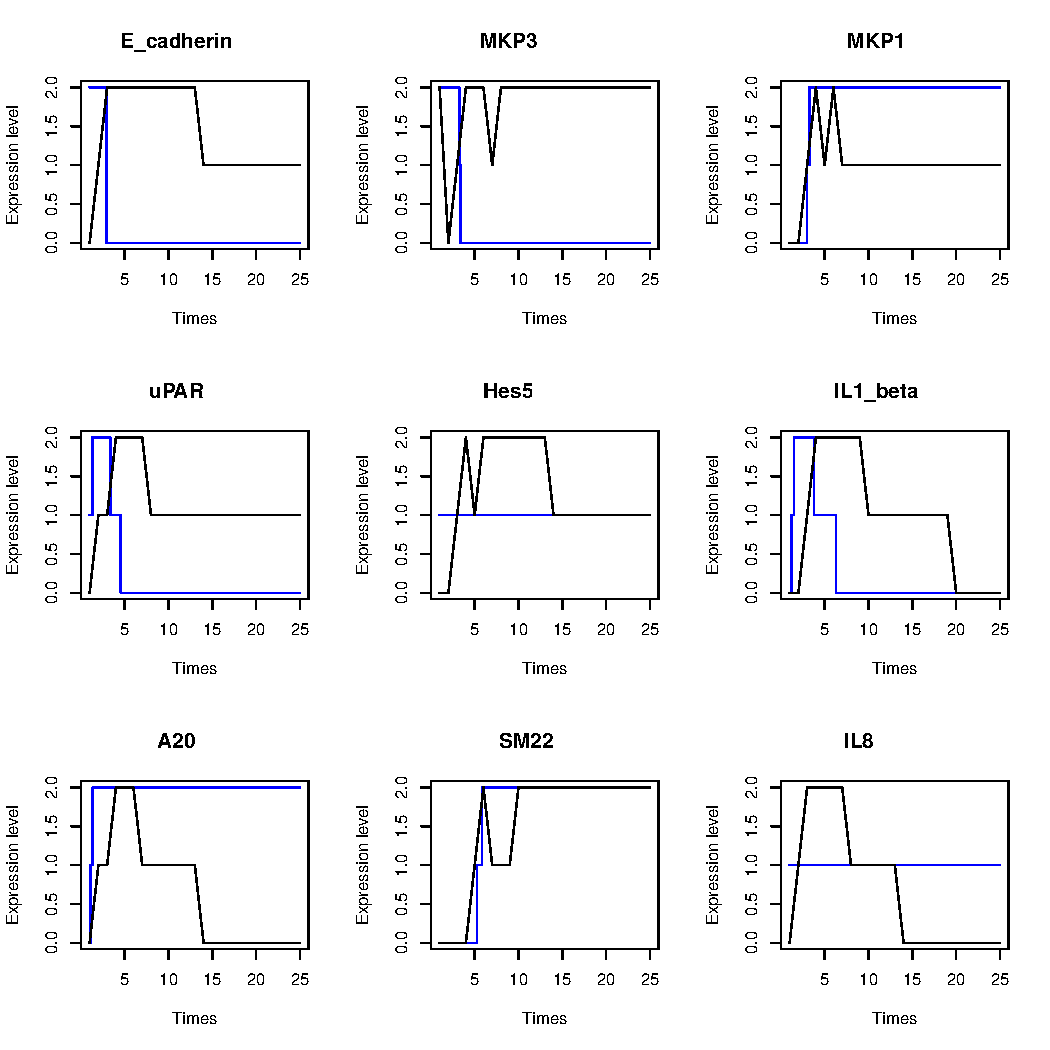
\includegraphics[width=6.5in,height=3.5in]{images/resultWS.pdf}
\caption{\bf Results of simulations by introducing the synchronization sort. In black line the expect behaviours
come from the discretization of time-series data. In Blue line the simulation behavior.}
\label{fig:rws}
\end{figure*}



% An example of a floating figure using the graphicx package.
% Note that \label must occur AFTER (or within) \caption.
% For figures, \caption should occur after the \includegraphics.
% Note that IEEEtran v1.7 and later has special internal code that
% is designed to preserve the operation of \label within \caption
% even when the captionsoff option is in effect. However, because
% of issues like this, it may be the safest practice to put all your
% \label just after \caption rather than within \caption{}.
%
% Reminder: the "draftcls" or "draftclsnofoot", not "draft", class
% option should be used if it is desired that the figures are to be
% displayed while in draft mode.
%
%\begin{figure}[!t]
%\centering
%\includegraphics[width=2.5in]{myfigure}
% where an .eps filename suffix will be assumed under latex, 
% and a .pdf suffix will be assumed for pdflatex; or what has been declared
% via \DeclareGraphicsExtensions.
%\caption{Simulation Results}
%\label{fig_sim}
%\end{figure}

% Note that IEEE typically puts floats only at the top, even when this
% results in a large percentage of a column being occupied by floats.


% An example of a double column floating figure using two subfigures.
% (The subfig.sty package must be loaded for this to work.)
% The subfigure \label commands are set within each subfloat command, the
% \label for the overall figure must come after \caption.
% \hfil must be used as a separator to get equal spacing.
% The subfigure.sty package works much the same way, except \subfigure is
% used instead of \subfloat.
%
%\begin{figure*}[!t]
%\centerline{\subfloat[Case I]\includegraphics[width=2.5in]{subfigcase1}%
%\label{fig_first_case}}
%\hfil
%\subfloat[Case II]{\includegraphics[width=2.5in]{subfigcase2}%
%\label{fig_second_case}}}
%\caption{Simulation results}
%\label{fig_sim}
%\end{figure*}
%
% Note that often IEEE papers with subfigures do not employ subfigure
% captions (using the optional argument to \subfloat), but instead will
% reference/describe all of them (a), (b), etc., within the main caption.


% An example of a floating table. Note that, for IEEE style tables, the 
% \caption command should come BEFORE the table. Table text will default to
% \footnotesize as IEEE normally uses this smaller font for tables.
% The \label must come after \caption as always.
%
%\begin{table}[!t]
%% increase table row spacing, adjust to taste
%\renewcommand{\arraystretch}{1.3}
% if using array.sty, it might be a good idea to tweak the value of
% \extrarowheight as needed to properly center the text within the cells
%\caption{An Example of a Table}
%\label{table_example}
%\centering
%% Some packages, such as MDW tools, offer better commands for making tables
%% than the plain LaTeX2e tabular which is used here.
%\begin{tabular}{|c||c|}
%\hline
%One & Two\\
%\hline
%Three & Four\\
%\hline
%\end{tabular}
%\end{table}


% Note that IEEE does not put floats in the very first column - or typically
% anywhere on the first page for that matter. Also, in-text middle ("here")
% positioning is not used. Most IEEE journals/conferences use top floats
% exclusively. Note that, LaTeX2e, unlike IEEE journals/conferences, places
% footnotes above bottom floats. This can be corrected via the \fnbelowfloat
% command of the stfloats package.

\section{Conclusion}
This work describes the steps towards the integration of time-series data in large-scale cell-based models. 
We proposed an automatic method to build a stochastic pi-calculus PH model from a biological system composed of biochemical reactions, extracted automatically from public databases, 
relevant to keratinocyte stimulation induced by Calcium. 
We then proposed a method to discretize time-series gene expression data, so they can be confronted to the PH simulations and logically explained by the PH static analyses. 
Finally we described a method to automatically estimate the temporal and stochastic
parameters for the PH simulation, so this estimation process will not be biased by over fitting. Ours results show that: (1) we reproduce accuretely in mean 
$7$ out of $12$ of the genes, (2) we can modele large scale networks in which signal goes from an input node to the output nodes, (3) we can reproduce tendences of the dynamic of components
and take in to accout the stochastic and time aspect of the bihaviours of the biological system.
As concrete perspectives of this work, we intend to \emph{(i)} validate the RSTC network topology by confronting its \emph{in-silico} simulation with real measurements of its components;
\emph{(ii)} compare the stochastic simulation results with reachability static analysis over the same PH components mapped to the $12$ measured genes; and 
finally \emph{(iii)} search for key-regulators up-stream the $12$ genes which will control the dynamics of the system, to  provide our biological partners concrete 
hypotheses to test experimentally.


%%%%%%%%%%%%%%%%%%%%%%%%%%%%%%%%%%%% put bibliographie here

\bibliographystyle{IEEEtran}
\bibliography{biblio.bib}


%\begin{thebibliography}{1}

%\bibitem{IEEEhowto:kopka}
%H.~Kopka and P.~W. Daly, \emph{A Guide to \LaTeX}, 3rd~ed.\hskip 1em plus
%  0.5em minus 0.4em\relax Harlow, England: Addison-Wesley, 1999.

%\end{thebibliography}




% that's all folks
\end{document}


